%*****************************************************************
%*************************** Section 4 ***************************
%********************* Antrieb des Fahrzeugs *********************
%*****************************************************************


\pagestyle{fancy}
\rhead{\thepage} \chead{} \lhead{\ref{Sec4}. \nameref{Sec4}}
\cfoot{}

\section{Antrieb des Fahrzeugs}\label{Sec4}

Wie in Kapitel \ref{Sec2Sub1} beschrieben, wird das Fahrzeug von zwei \acp{BLDCMot} angetrieben, die im Folgenden genauer erklärt werden. Zusätzlich dazu wird in diesem Kapitel auch näher auf die Montage der Antriebskomponenten, die Programmierung des Antriebsbausteins, die Konfiguration der Motorcontroller und die Drehzahlmessung eingegangen.

\subsection{BLDC-Antrieb und Motorcontroller}\label{Sec4Sub1}

\acp{BLDCMot} sind im Wesentlichen wie permanent erregte Synchronmaschinen aufgebaut. Sie besitzen Magnete im Rotor und Einzelzahnwicklungen im Stator. Da solche Motoren häufig im \ac{RC}-Bereich Einsatz finden, gibt es zu deren Ansteuerung bereits vorgefertigte Bausteine, sogenannte \ac{ESC}. Diese haben zwei Signalpins für ein \ac{PWM}-Signal und zwei Anschlüsse zur Spannungsversorgung des Motorcontrollers, aus welchen die drei Strangspannungen für die Phasen des Antriebs generiert werden. Aus diesen Strangspannungen kann im übrigen auch die Motordrehzahl ermittelt werden, was im Rahmen dieser Projektarbeit auch eines der Ziele darstellt. An den Signalpins wird ein \ac{PWM}-Signal mit einer Frequenz von 50Hz angelegt, dessen Pulsbreite zwischen 1ms und 2ms liegen darf. Daraus resultiert ein Tastgrad zwischen 5\% (Stillstand) und 10\% (maximal erreichbare Drehzahl). Die maximale Drehzahl des Antriebs hängt von der Spannung des Akkus ab. Je geringer diese Spannung ist, desto geringer ist die maximal erreichbare Drehzahl. Der Anschluss der Motoren erfolgt nach der in Abbildung \ref{fig:SkizzeAntrieb} gezeigten Weise.

\begin{figure}[H] %H für Positionierung hier
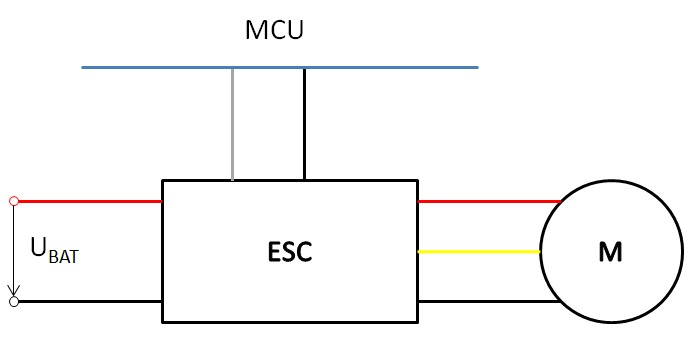
\includegraphics[width=.90\textwidth]{sec4/images/Skizze_BLDC_ESC} 
\centering
\captionsetup{width=.95\textwidth}
\caption[Skizze zur Beschaltung eines \ac{ESC}s und \ac{BLDCMot}s]{Skizze zur Beschaltung eines \ac{ESC}s und \ac{BLDCMot}s; Versorgungsspannung des \ac{ESC}s in rot und schwarz (Masse), \ac{PWM}-Signalleitungen in grau und schwarz (Masse) und Anschlussleitungen des \ac{BLDCMot}s in rot, gelb und schwarz}\centering
\label{fig:SkizzeAntrieb}
\end{figure}

\subsection{Montage der Antriebskomponenten}\label{Sec4Sub2}

Die Komponenten des Fahrzeugantriebs, welcher über zwei \acp{BLDCMot} realisiert ist, sind auf der unteren Fahrzeugebene montiert. Die Motoren selbst sind mit zwei Schrauben an der Karosserie befestigt. An der Welle der Motoren befindet sich je ein Zahnrad mit 13 Zähnen, welches ein weiteres Zahnrad mit 90 Zähnen antreibt, das an der Antriebswelle befestigt ist. Das heißt, dass sich die Reifen bei 6,923 Umdrehungen der Motorwelle genau einmal drehen.\vspace{11pt}

In Abbildung \ref{fig:MontageMotorUebersetzung} sind die montierten Komponenten des linken Antriebs abgebildet. Die Befestigungsschrauben der Motoren sind dabei in rot hervorgehoben, die Befestigungsschrauben des Zahnrads der Antriebswelle in blau und die Befestigung des Reifens in orange. Das Zahnrad der Motorwelle ist durch Erhitzen geweitet und auf die Welle aufgesetzt worden. Zur Sicherheit dient hier etwas Sekundenkleber dazu, dass sich das Zahnrad auf der Welle nicht durchdreht. Sekundenkleber ist hier völlig ausreichend, da aufgrund der Übersetzung nur 1/7 des auf die Reifen wirkenden Moments auf das Zahnrad der Motorwelle wirkt.

\begin{figure}[H] %H für Positionierung hier
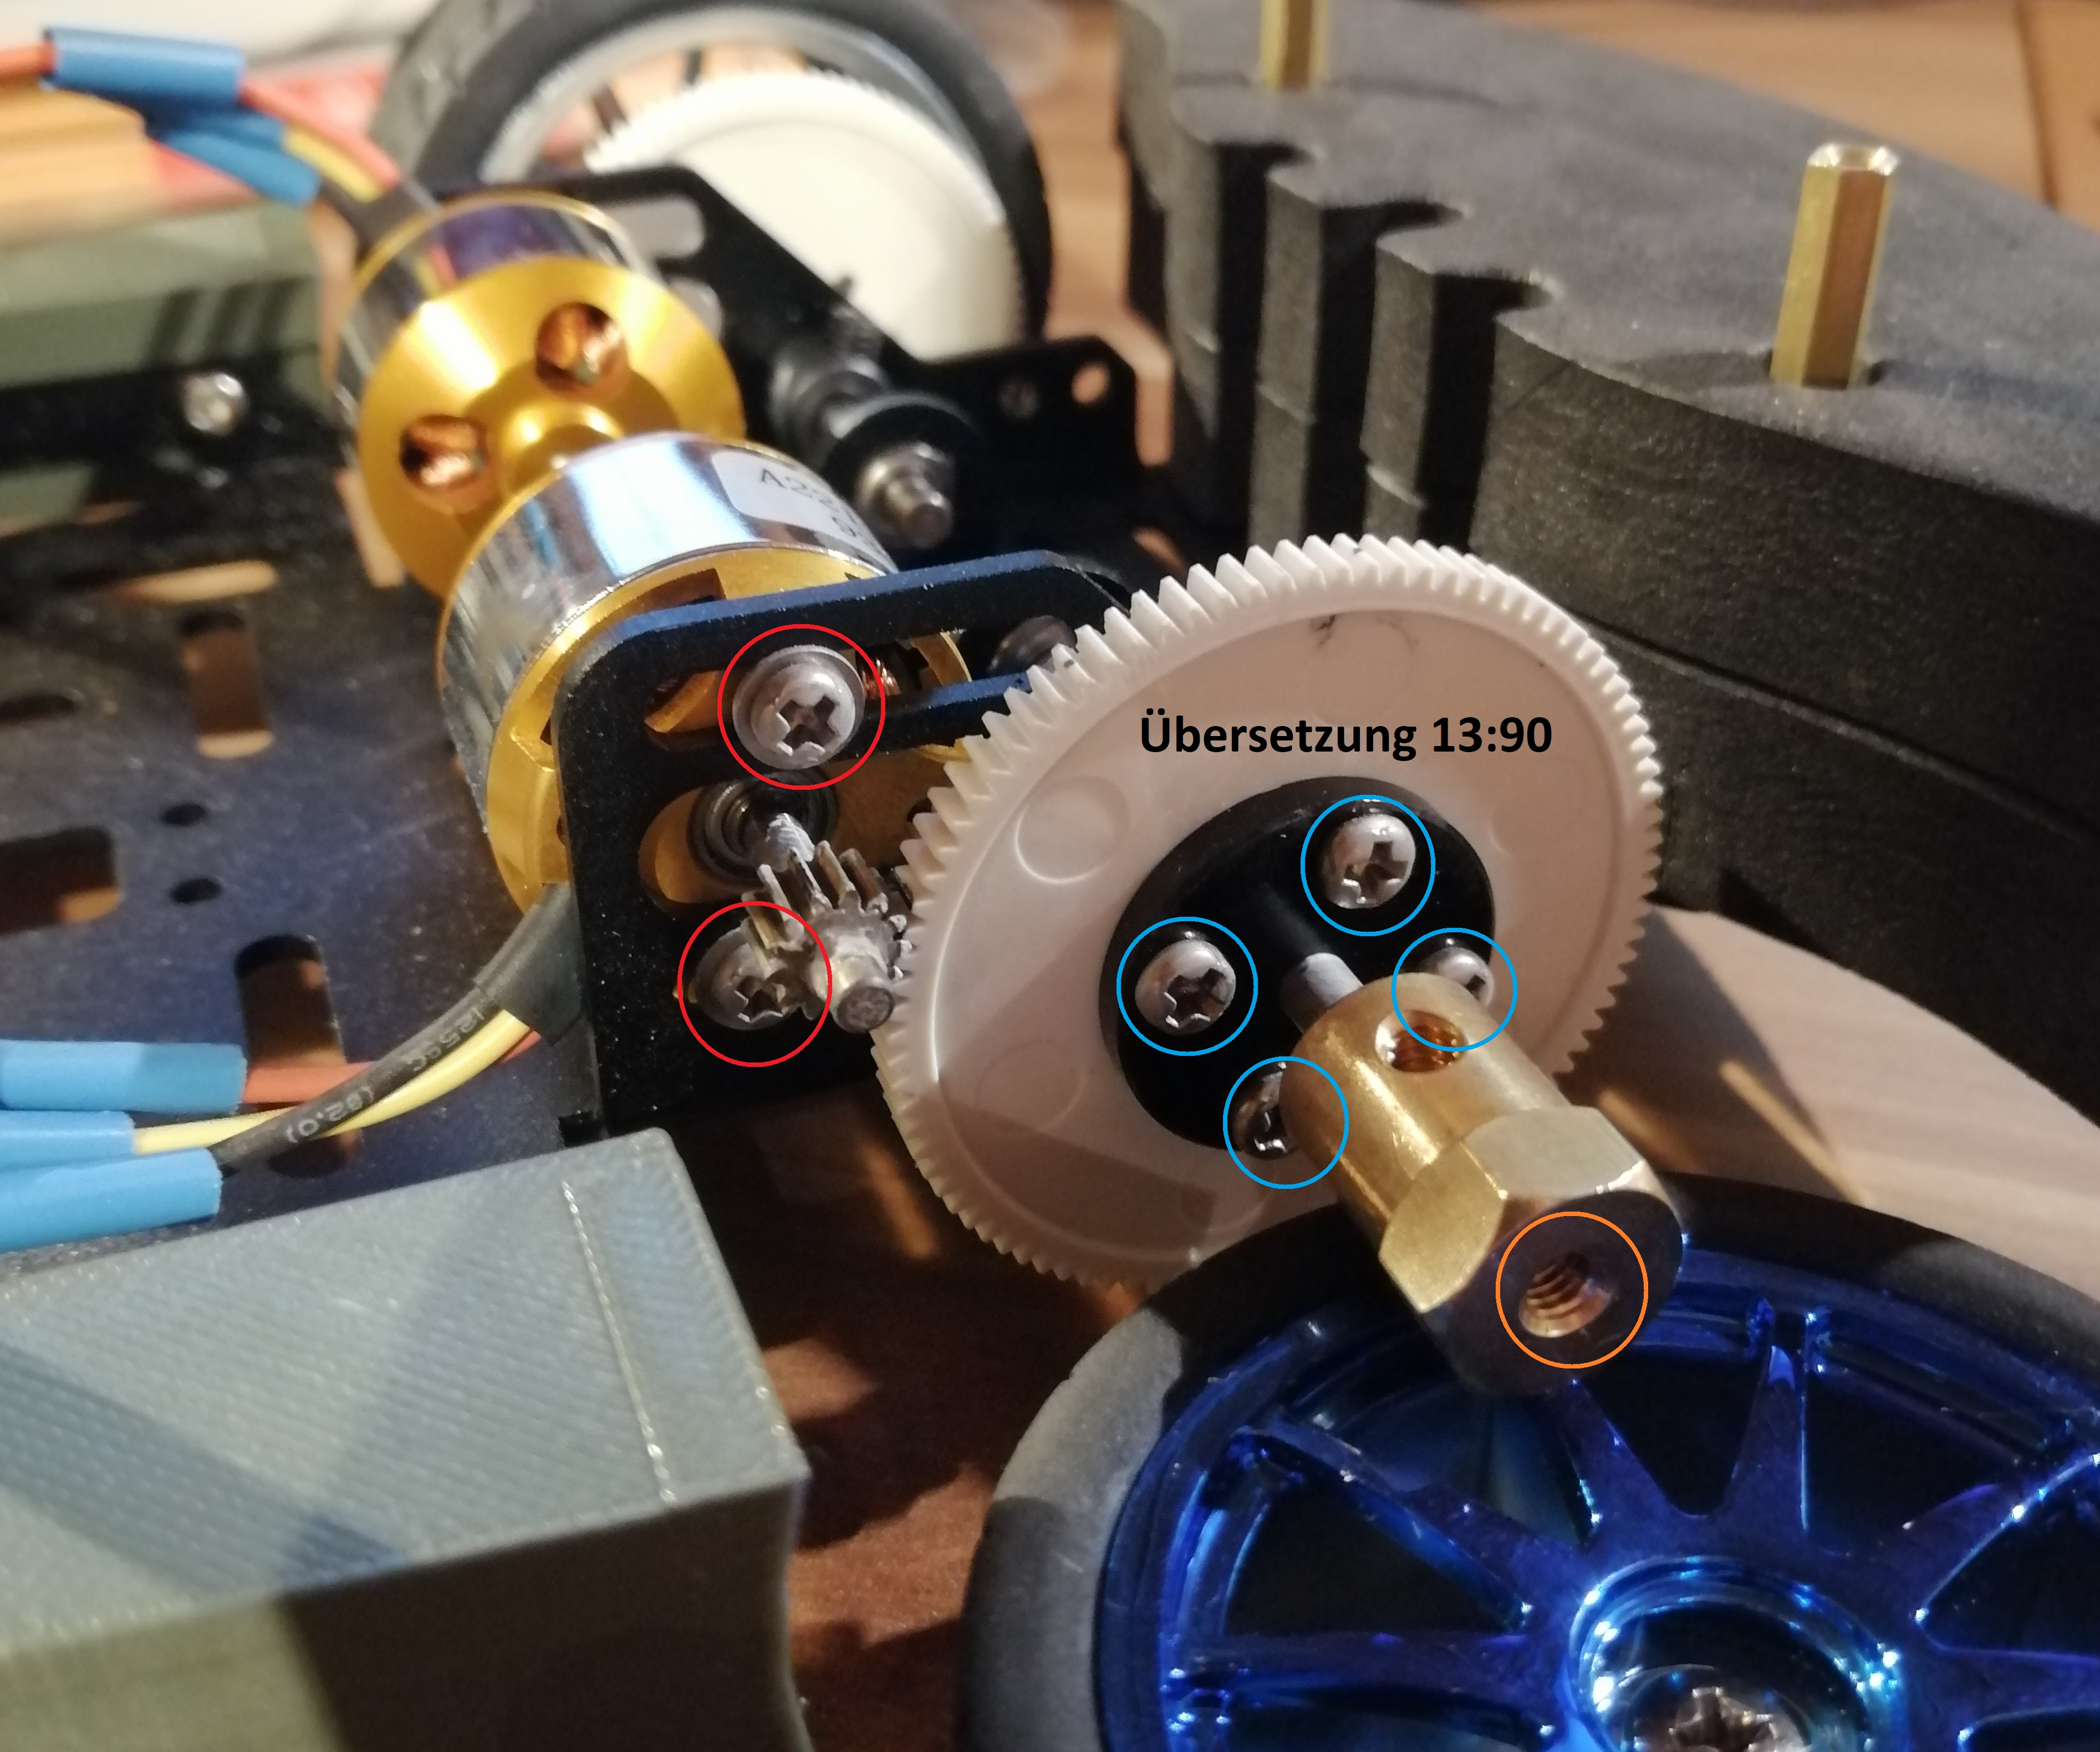
\includegraphics[width=.90\textwidth]{sec4/images/MontageMotorUebersetzung} 
\centering
\captionsetup{width=.95\textwidth}
\caption[Montage der Antriebskomponenten]{Montage der \acp{BLDCMot} und Übersetzung auf die Antriebsachse; In rot die Befestigung des \ac{BLDCMot}s, in blau die Befestigung des Zahnrads an der Antriebswelle und in orange die Befestigung des Reifens}\centering
\label{fig:MontageMotorUebersetzung}
\end{figure}

\subsection{Konfiguration der Motorcontroller}\label{Sec4Sub3}

Die beiden Motorcontroller erwarten nach dem Zuschalten der Spannungsversorgung eine Initialisierungssequenz. Das Power-On-Ereignis wird vom \ac{ESC} mit drei Tönen (tief, mittel, hoch) signalisiert. Im Anschluss daran soll der Wert an der Signalleitung größer als 0\% sein. Das bedeutet, dass ein \ac{PWM}-Signal angelegt werden muss, welches eine Drehzahl N $\geq$ 0rpm repräsentiert. Der \ac{ESC} quittiert das Erkennen des \ac{PWM}-Signals mit einem tiefen Ton. Die Initialisierungssequenz ist allerdings erst dann beendet, wenn das \ac{PWM}-Signal an der Signalleitung zuerst vergrößert und dann auf 0\% verringert wird (N = 0rpm). Dabei gibt der \ac{ESC} einen letzten, hohen Ton von sich. Der Ablauf der Initialisierungssequenz ist in Abbildung \ref{fig:initESC} dargestellt. Nach dem letzten Ton ist die Initialisierung beendet und der \ac{BLDCMot} dreht sich in Abhängigkeit des an der Signalleitung anliegenden \ac{PWM}-Signals. 

\begin{figure}[H] %H für Positionierung hier
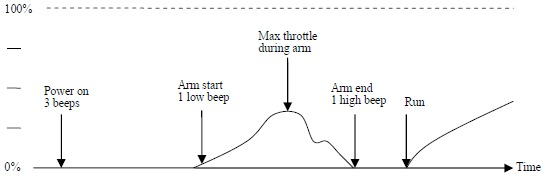
\includegraphics[width=.90\textwidth]{sec4/images/BLDCInit} 
\centering
\captionsetup{width=.95\textwidth}
\caption[Initialisierungssequenz der \ac{ESC}s]{Initialisierungssequenz der \ac{ESC}s; Wert an der Signalleitung für die Initialisierungssequenz über der Zeit; 0\% entspricht dem \ac{PWM}-Tastgrad für den Stillstand und 100\% dem für die maximal erreichbare Drehzahl}\centering
\label{fig:initESC}
\end{figure}

Da die \ac{ESC}s individuell konfiguriert werden können und in der Dokumentation zu wenige Angaben gemacht werden, ist der Tastgrad für die Werte 0\% (Stillstand) und 100\% (maximal erreichbare Drehzahl) unbekannt. Deshalb ist es nicht möglich zu wissen, welche \ac{PWM}-Tastgrade für die Initialisierungssequenz verwendet werden müssen. Über die Konfiguration der \ac{ESC}s können die Grenzen für 0\% und 100\% selbst festgelegt werden. Für das Flashen der Motorcontroller wird die Software \glqq{}BLHeliSuite\grqq{} verwendet. Die Verbindung zwischen den \ac{ESC}s und der Software stellt ein Arduino Nano her.\vspace{11pt}

Der Arduino Nano muss zuvor mit einer neuen Software beschrieben werden. Um die \ac{ESC}s flashen zu können wird der Signalpin des zu programmierenden \ac{ESC} mit dem Pin D3 und der Massepin der Signalleitung mit einem Massepin des Arduino Nano verbunden. Danach wird in der Software \glqq{}BLHeliSuite\grqq{} im Reiter \glqq{}Make Interface\grqq{} eine neue Schnittstelle erstellt (siehe Abbildung \ref{fig:ConfigBLHeliSuite}). Auf der rechten Seite des Programm-Fensters wird ein Arduino Nano als Schnittstelle eingerichtet. Mit einem Klick auf den Button \glqq{}Arduino 4way-interface\grqq{} wird die neue Software, durch die die \ac{ESC}s neu konfiguriert werden können, auf den Arduino Nano geladen.

\begin{figure}[H] %H für Positionierung hier
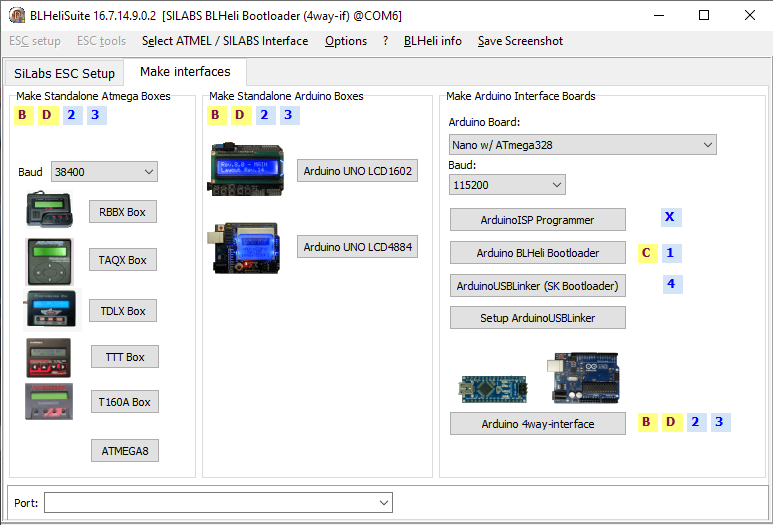
\includegraphics[width=.78\textwidth]{sec4/images/Config_BLHeliSuite} 
\centering
\captionsetup{width=.95\textwidth}
\caption[Programmierung des Arduino Nano zur \ac{ESC}-Konfiguration]{Programmierung des Arduino Nano zur \ac{ESC}-Konfiguration mit der Software BLHeliSuite}\centering
\label{fig:ConfigBLHeliSuite}
\end{figure}

Nach dem Programmieren des Arduino Nano wird die Kommunikation der BLHeliSuite-Software mit dem \ac{ESC} hergestellt. Über die Schaltfläche \glqq{}Read Setup\grqq{} werden die voreingestellten Parameter des \ac{ESC} ausgelesen. Im nächsten Schritt werden die Zeiten für die Werte \glqq{}PPM min Throttle\grqq{} (0\% Aussteuergrad) und \glqq{}PPM max Throttle\grqq{} (100\% Aussteuergrad) auf 1100µs und 1900µs angepasst. Alle vorgenommenen Einstellungen sind in Abbildung \ref{fig:BLHeliSuite} einsehbar. Die Werte werden über die Betätigung der Schaltfläche \glqq{}Write Setup\grqq{} auf den \ac{ESC} geladen. Da jetzt die Werte für 0\% und 100\% Aussteuerung bekannt sind, können die einzelnen Schritte der Initialisierung im Programm des Fahrzeugs abgearbeitet werden.

\begin{figure}[H] %H für Positionierung hier
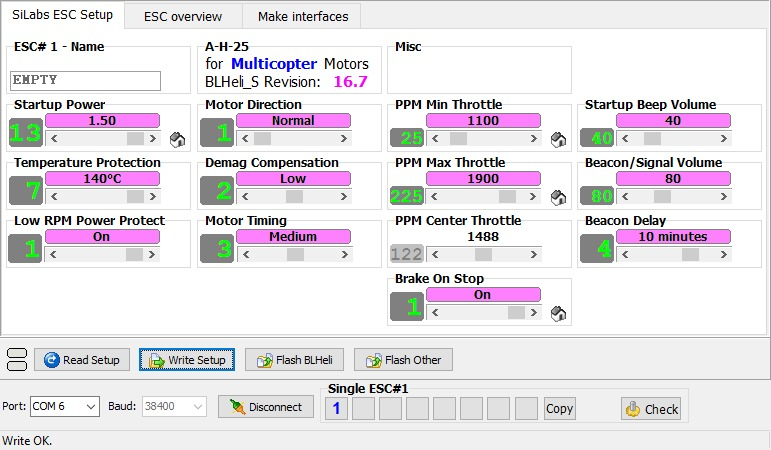
\includegraphics[width=.78\textwidth]{sec4/images/ESC_config} 
\centering
\captionsetup{width=.95\textwidth}
\caption[Parameter der neuen \ac{ESC}-Konfiguration]{Konfiguration der \ac{ESC}s mit der Software \glqq{}BLHeliSuite\grqq{}}\centering
\label{fig:BLHeliSuite}
\end{figure}

\subsection{Programmierung des Antriebsbausteins}\label{Sec4Sub4}

Der Antriebsbaustein der Software ist in zwei Dateien unterteilt, die Dateien \glqq{}drive.c\grqq{} und \glqq{}drive.h\grqq{}. Die Datei \glqq{}drive.h\grqq{} enthält alle relevanten Bibliotheken und Prototypen für die Datei \glqq{}drive.c\grqq{}.\vspace{11pt}

Außer der Einbindung der Bibliotheken und der Prototypen der Funktionen aus der Datei \glqq{}drive.c\grqq{} sind hier auch die Parameter für die Initialisierungssequenz der \ac{ESC}s und für die Initialisierung des Timers für die \ac{PWM}-Signale hinterlegt (Abbildung \ref{fig:DriveH}). 

\begin{figure}[H] %H für Positionierung hier
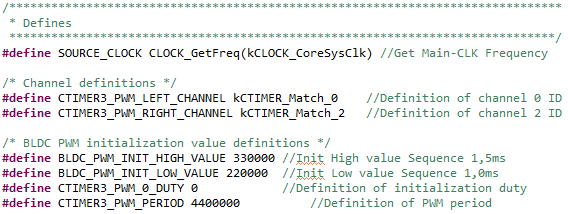
\includegraphics[width=.85\textwidth]{sec4/images/DriveH} 
\centering
\captionsetup{width=.95\textwidth}
\caption[Relevante Zeilen der Datei \glqq{}drive.h\grqq{}]{Relevante Zeilen der Datei \glqq{}drive.h\grqq{} mit den Parametern für die Initialisierungssequenz der \ac{ESC}s und für die Initialisierung des \ac{PWM}-Timers}\centering
\label{fig:DriveH}
\end{figure}

Für die \ac{PWM}-Periodendauer wird bei der Initialisierung ein Wert von 4.400.000 Takten festgesetzt, woraus mit einer \ac{CPU}-Taktfrequenz von 220MHz (220.000.000 Takte pro Sekunde) eine Periodendauer von 20ms resultiert. Die Pulsbreite wird während des Programmablaufs regelmäßig überschrieben.\vspace{11pt}

Der \ac{ESC}-Initialisierungswert für den Stillstand (\glqq{}BLDC\_PWM\_INIT\_LOW\_VALUE\grqq{}, 220.000) entspricht hier einer \ac{PWM}-Pulsbreite von 1,0ms und der Initialisierungswert für die in etwa mittlere Aussteuerung (\glqq{}BLDC\_PWM\_INIT\_HIGH\_VALUE\grqq{}, 330.000) einer Breite von 1,5ms. Die volle Aussteuerung der Motoren wird, wie über die \glqq{}BLHeliSuite\grqq{} festgelegt, bei einer Pulsdauer von 1,9ms erreicht (BLDCMaxValue, ca. 418.000). Eine Drehzahl von N = 0rpm wird theoretisch über die bei der \ac{ESC}-Konfiguration festgelegten 1,1ms ermöglicht (242.000). Da das \ac{PWM}-Signal leicht abweicht, wird ein etwas geringerer Wert veranlagt (BLDCMaxValue, ca. 240.000 = 1,09ms). Damit wird sichergestellt, dass sich die Räder im Stillstand nicht drehen.\vspace{11pt}

Die Parameter BLDCMaxValue und BLDCMinValue existieren im Code für die linke und rechte Antriebsseite separat (\glqq{}BLDCLeftMaxValue\grqq{}, \glqq{}BLDCLeftMinValue\grqq{} \& \glqq{}BLDCRightMaxValue\grqq{}, \glqq{}BLDCRightMinValue\grqq{}). Die Werte dieser Parameter kommen direkt aus dem \ac{EEPROM} und können mit dem Bedienungsboard eingestellt werden (siehe Abbildung \ref{fig:DriveC0}).\vspace{11pt}

\begin{figure}[H] %H für Positionierung hier
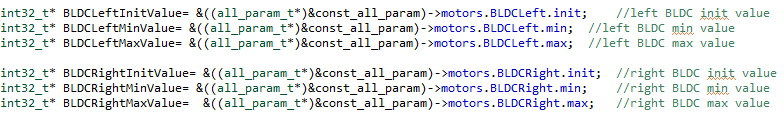
\includegraphics[width=.95\textwidth]{sec4/images/DriveC0} 
\centering
\captionsetup{width=.95\textwidth}
\caption[Extremwerte der Antriebsgeschwindigkeit als Parameter aus dem \ac{EEPROM}]{Extremwerte der Antriebsgeschwindigkeit als Parameter aus dem \ac{EEPROM}, deren Werte über das Bedienungsboard individuell einstellbar sind; Teil der Datei \glqq{}drive.c\grqq{}}\centering
\label{fig:DriveC0}
\end{figure}

Auch die beiden \ac{PWM}-Timer (einer je Motorcontroller) benötigen bei der Initialisierung einige Parameter, deren Werte in der Datei \glqq{}drive.h\grqq{} festgelegt sind (PWM-Periodendauer, \ac{PWM}-Pulsdauer, Channel). Die Channel werden auf das Timer Match Register 2 (rechter Antrieb, \glqq{}kCTIMER\_Match\_2\grqq{}) und auf das Timer Match Register 0 (linker Antrieb, \glqq{}kCTIMER\_Match\_0\grqq{}) festgelegt, was bei dem verwendeten Controller den Pins P0.27 (rechts) und P3.10 (links) entspricht. Der Pin P3.10 wird auf der Controllerplatine über den Pin 7 und der Pin P0.27 über den Pin 12 der Buchsenleiste J13 nach außen geführt. Der Anschluss der Motorcontroller ist über den Anhang \glqq{}\nameref{SecAtt1}\grqq{} nachvollziehbar.\vspace{11pt}

\begin{figure}[H] %H für Positionierung hier
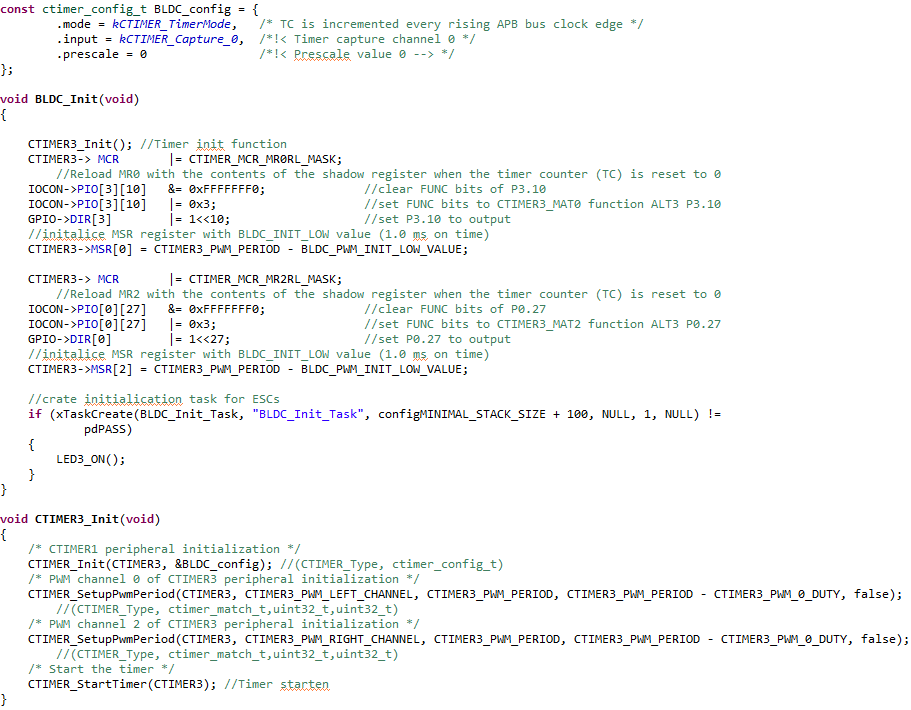
\includegraphics[width=.95\textwidth]{sec4/images/DriveC1} 
\centering
\captionsetup{width=.95\textwidth}
\caption[Funktionen BLDC\_Init und CTIMER3\_Init der Datei \glqq{}drive.c\grqq{}]{Funktionen BLDC\_Init und CTIMER3\_Init der Datei \glqq{}drive.c\grqq{}}\centering
\label{fig:DriveC1}
\end{figure}

Die Datei \glqq{}drive.c\grqq{} enthält die Funktionen zur Initialisierung der für die Verwendung der Antriebe notwendigen Controller-Peripherie (siehe Abbildung \ref{fig:DriveC1}) und zur Initialisierung der Motorcontroller (siehe Abbildung \ref{fig:DriveC2}).\vspace{11pt}

In der Funktion BLDC\_Init wird zuerst die Funktion CTIMER3\_Init aufgerufen, welche die beiden vorher festgelegten Kanäle des Timers C3 (\glqq{}kCTIMER\_Match\_0\grqq{} und \glqq{}kCTIMER\_Match\_2\grqq{}) mit den in der Datei ''drive.h'' festgelegten Parametern als \ac{PWM}-Timer mit einer Periodendauer von 20ms und einer Pulsdauer von 0ms initialisiert. Im Anschluss daran wird einzeln für beide Kanäle festgelegt, dass bei einem Timer-Überlauf die neuen Daten für die Pulslängen aus den Shadow-Registern geladen werden sollen. Zum Ändern der Geschwindigkeit eines der beiden Antriebe muss deshalb lediglich ein neuer Wert in das Shadow-Register geschrieben werden. Hier muss allerdings aufgepasst werden, da das Register nicht die Pulsbreite (On-Time) sondern die Off-Time erwartet. Deshalb muss der Wert, der eingetragen wird, der Periodendauer abzüglich der Pulsdauer entsprechen. Zusätzlich werden in der Funktion BLDC\_Init auch die Pins P3.10 und P0.27 für die Verwendung als \ac{PWM}-Ausgang des Timers C konfiguriert. Am Ende wird noch der erste \ac{ESC}-Initialisierungswert in die beiden Shadow-Register geschrieben, bevor die \ac{ESC}-Initialisierungsfunktion aufgerufen wird (siehe Abbildung \ref{fig:DriveC2}).

\begin{figure}[H] %H für Positionierung hier
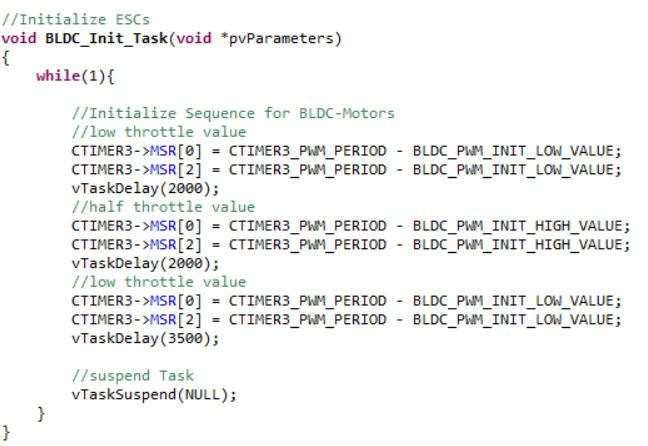
\includegraphics[width=.9\textwidth]{sec4/images/DriveC2} 
\centering
\captionsetup{width=.95\textwidth}
\caption[Funktion BLDC\_Init\_Task der Datei \glqq{}drive.c\grqq{}]{Funktion BLDC\_Init\_Task der Datei \glqq{}drive.c\grqq{} zum Durchlaufen der Initialisierungssequenz der \ac{ESC}s}\centering
\label{fig:DriveC2}
\end{figure}

Der Task BLDC\_Init\_Task beginnt mit dem Befüllen der Shadow-Register mit dem ersten Initialisierungswert. Nach einer Wartezeit von 2s wird der zweite Initialisierungswert in die Register geschrieben. Ebenfalls nach einer Zeit von 2s wird dann wieder der erste Initialisierungswert in die Shadow-Register geschrieben und die Initialisierung der \ac{ESC}s ist abgeschlossen. Die Wartezeiten sind notwendig, damit die \ac{ESC}s Zeit haben, die Änderungen zu erfassen.



\newpage
\subsection{Drehzahlmessung}\label{Sec4Sub5}

\subsubsection{Erörterung der Notwendigkeit einer Drehzahlmessung}\label{Sec:NotwendigkeitDrehzahlmessung}

Die Quellspannung von Akkus verringert sich mit steigender Betriebszeit, weshalb bereits bei vorherigen Fahrzeug-Versionen eine Drehzahlmessung benötigt wurde, um über eine Regelung die Spannungsabhängigkeit der Drehzahl bei \acp{DCMot} ausgleichen zu können. Die Spannungsabhängigkeit hat insbesondere beim Überfahren eines Hügels Probleme bereitet. Da die in den vorangegangenen Fahrzeugmodellen verwendeten \acp{DCMot} durch \acp{BLDCMot} ersetzt wurden, stellt sich allerdings erneut die Frage nach der Notwendigkeit einer Drehzahlmessung. Die Variation der Drehzahl erfolgt bei \acp{DCMot} über die Änderung der Betriebsspannung, was auch die Abhängigkeit von der Versorgungsspannung erklärt. Die Drehzahlvariation bei einem \ac{BLDCMot} wird hingegen über eine Frequenzänderung der Strangspannungen realisiert. Zur Klärung der Frage nach einer Spannungsabhängigkeit der \acp{BLDCMot}, ist eine Messung am Prüfstand erforderlich.\vspace{11pt}

	Für die Durchführung der Messung wird ein bereits vorhandener Prüfstand für Modellfahrzeuge verwendet, welcher im Rahmen einer Bachelor-Abschlussarbeit an der HAW Landshut erstellt wurde. Für die Durchführung wird ein in Abbildung \ref{fig:Pruefstand01} zu sehender, bereits vorhandener, Messaufbau verwendet. Damit das Fahrzeug möglichst stabil auf dem Prüfstand steht und die Räder des Fahrzeuges einen besseren Halt bekommen, wird mit Hilfe eines Drahtes das Heck des Fahrzeugs am Prüfstand befestigt (siehe Abbildung 44 blaue Markierung). Die vorderen Räder des Fahrzeuges sind ebenfalls mit einem am Prüfstand integrierten Befestigungsmechanismus befestigt (siehe Abbildung 44 gelbe Markierungen). \vspace{11pt}

Zur Überprüfung einer eventuellen Abhängigkeit der Drehzahl von der Versorgungsspannung, wird die Spannung an den vorhandenen \acp{DCMot} des Prüfstands gemessen, da diese direkt proportional zur Drehzahl ist (siehe Gleichung \ref{eq1}). Die Abhängigkeit der gemessenen Spannung von der Drehzahl ist allerdings nur annähernd linear, da die Drehmomentkonstante k\textsubscript{i} bei hohen Drehzahlen leicht einbricht. Aufgrund der für die Messung konstant eingestellten Pulsbreite von 1,5ms, spielt der Einbruch der Drehmomentkonstante allerdings keine große Rolle, da sich die Drehzahl wenn überhaupt nur sehr gering ändert. Dieser Zusammenhang kann deshalb vereinfachend als linear angenommen werden.


\begin{figure}[H] %H für Positionierung hier
\includegraphics[width=.80\textwidth]{sec4/images/Pruefstand_Messung_UAbhängigkeit} 
\centering
\captionsetup{width=.95\textwidth}
\caption[Messaufbau zur Prüfung der Spannungsabhängigkeit der \acp{BLDCMot}]{Messaufbau zur Prüfung der Spannungsabhängigkeit der \acp{BLDCMot}; in blau die Befestigung des Hecks an der Grundplatte des Prüfstands, in gelb die Befestigung der Vorderreifen am Prüfstand, in rot die DC-Motoren zur Spannungsmessung}\centering
\label{fig:Pruefstand01}
\end{figure}

Die Versorgungsspannung der \acp{ESC} wird für die Aufnahme verschiedener Messwerte zwischen 6,1V und 8V variiert. Ändert sich die gemessene Spannung mit der Variation der Versorgungsspannung, so ist das ein hinreichender Beweis dafür, dass die Drehzahl der \acp{BLDCMot} spannungsabhängig ist. Die Ergebnisse der Messreihe aus Tabelle \ref{tab:PruefstandMess01} sind zur einfacheren Auswertung in Abbildung \ref{fig:Pruefstand02} visualisiert.

\begin{equation}\label{eq1}
U_A = k_i \cdot N \cdot \frac{\pi}{30}
\end{equation}

\begin{table}[H]
\begin{tabular}{|c|c|c|c|c|c|c|c|c|c|c|}
\hline
\rule{0pt}{15pt} Messung & 1&2&3&4&5&6&7&8&9&10 \\
\hline
U\textsubscript{Versorgung} [$V$]&8.0&7.9&7.8&7.7&7.6&7.5&7.4&7.3&7.2&7.1 \\ 
\hline
U\textsubscript{Messung} [$V$]&5.80&5.75&5.65&5.57&5.48&5.40&5.35&5.25&5.18&5.09 \\
\hline
\hline
\rule{0pt}{15pt} Messung & 11&12&13&14&15&16&17&18&19&20 \\
\hline
U\textsubscript{Versorgung} [$V$]&7.0&6.9&6.8&6.7&6.6&6.5&6.4&6.3&6.2&6.1 \\ 
\hline
U\textsubscript{Messung} [$V$]&5.05&4.96&4.87&4.82&4.69&4.73&4.66&4.60&4.50&4.45 \\
\hline
\end{tabular}
\centering
\captionsetup{width=.95\textwidth}
\caption[Messreihe 1: Spannungsabhängigkeit Drehzahl]{Messreihe 1: Messwerte für Überprüfung einer eventuellen Spannungsabhängigkeit der Drehzahl}\centering
\label{tab:PruefstandMess01}
\end{table}

Aus Abbildung \ref{fig:Pruefstand02} können einige wertvolle Erkenntnisse abgeleitet werden. Zum einen ist die Drehzahl, welche proportional zu der an den \ac{DCMot} gemessenen Ankerspannung U\textsubscript{Messung} ist, nicht konstant. Zum anderen ist die Drehzahl der \acp{BLDCMot} von der Versorgungsspannung der \acp{ESC} abhängig, denn andernfalls wäre die resultierende Gerade eine Horizontale.\vspace{11pt}

Die sich aus der Messreihe ergebenden Erkenntnisse, führen zu dem Entschluss, dass eine Drehzahlregelung nicht nur sinnvoll, sondern auch erforderlich ist. Denn während der Durchfahrt des Parcours wird nicht zu jedem Zeitpunkt die volle Drehzahl benötigt. Folglich würde das Fahrzeug bei stärkerer Kurvenfahrt über den Streckenrand hinaus fahren. Jedes Verlassen des Streckenrandes würde im Zuge des NXP-Cups eine Strafzeit von einer Sekunde bedeuten. Zusätzlich hat eine Regelung den Vorteil, dass die vorgegebene Drehzahl auch bei einer fortschreitenden Entladung des Akkus weiterhin aufrecht gehalten werden kann. Wird eine feste Geschwindigkeit vorgegeben, kann die Regelung bei fallender Versorgungsspannung der \acp{ESC} das \ac{PWM}-Signal bis zur Stellgrenze (Pulsbreite = 1,9ms) erhöhen. Erst bei Erreichen der Stellgrenze nimmt die Drehzahl linear mit der Versorgungsspannung ab.


\begin{figure}[H] %H für Positionierung hier
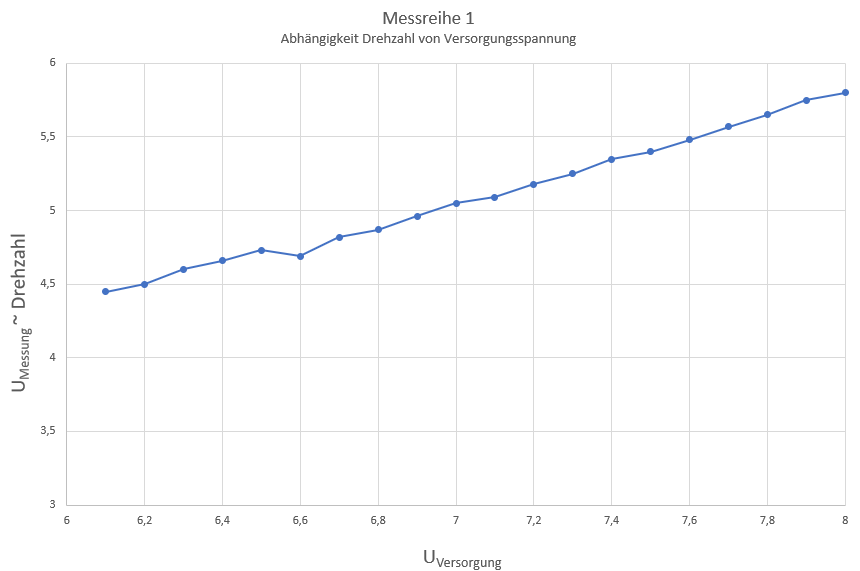
\includegraphics[width=.90\textwidth]{sec4/images/PruefstandMess02} 
\centering
\captionsetup{width=.95\textwidth}
\caption [Diagramm 1: Spannungsabhängigkeit Drehzahl]{Darstellung der Messwerte zur Spannungsabhängigkeit der Drehzahl in einem Diagramm}\centering
\label{fig:Pruefstand02}
\end{figure}

Des weiteren muss das Fahrzeug im Rahmen des NXP-Cups nach dem Überfahren der Ziellinie innerhalb von zwei Metern anhalten können. In der Konfiguration der \acp{ESC} bietet sich dafür die Einstellung \glqq{}Break On Stop\grqq{} an, mit der das Fahrzeug bei einer PWM-Pulsdauer von 1ms (STOPTHROTTLE) aktiv bremst, indem die drei Phasen der \acp{BLDCMot} auf Masse geschlossen werden.\vspace{11pt}

Zur Verifizierung eines ordnungsgemäßen Bremsverhaltens, wird eine Probefahrt auf einer langen geraden Strecke an der HS-Landshut durchgeführt. Die Antriebe sind dabei so konfiguriert das sich das Fahrzeug nach der Initialisierung der \acp{BLDCMot} unmittelbar mit maximalen Antrieb fortbewegt und nach kurzer Fahrt (ca. 5 m) in den \glqq{}STOPTHROTTLE\grqq{} Modus übergeht. Hierbei stellt man fest, dass die Bremskraft ausreicht, um das Fahrzeug innerhalb von ca. 30 cm zum Stehen zu bringen. Allerdings kann auch festgestellt werden, dass das Fahrzeug während des Bremsvorgangs wegrutscht und in allen Versuchen quer zum stehen kommt. Der genaue Grund für dieses Problem kann zu diesem Zeitpunkt nicht explizit festgestellt werden.\vspace{11pt}

Zur Überprüfung dieser Problematik wird das Fahrzeug wiederholt auf den vorhandenen Modellprüfstand gestellt und mit verschiedenen Geschwindigkeiten angesteuert. Insbesondere bei \glqq{}STOPTHROTTLE\grqq{} und sehr langsamer Fahrt (Pulsbreite 1,09ms - 1,20ms) kann festgestellt werden, dass der rechte BLDC-Motor nicht oder nur ruckartig dreht, während der linke BLDC-Motor einwandfrei läuft. Da die ESC-Konfiguration für beide \acp{BLDCMot} exakt gleich durchgeführt worden ist, kann man darauf schließen das es hier zu einem  Problemen im Antriebsmechanismus kommt. Aufgrund der mehrfachen Übersetzung zwischen \acp{BLDCMot} und Rädern durch entsprechende Zahnräder, wird davon ausgegangen, dass Reibungseffekte das Drehen der Motoren unterschiedlich bremsen bzw. beeinflussen. Zusätzlich kann auch die unterschiedlich feste Montage der Räder eine Ursache für dieses Verhalten darstellen.
%Zum anderen wird davon ausgegangen, dass bei minimalen und maximalen Antrieb die Stellgrenzen (1,09ms und 1,9ms) sprich die ON-Zeit des PWM-Signals kurzfristig über- bzw. unterschritten wird. Befindet sich die Pulsbreite außerhalb des konfigurierten Bereiches schaltet der Antrieb kurzweilig aufgrund des undefinierten Signalzustandes ab und bei Rückkher in den definierten Bereich wieder an.\vspace{11pt} 

Die vom NXP-Cup vorgegebenen Regularien, die Spannungsabhängigkeit der \acp{BLDCMot} sowie das unterschiedliche Drehverhalten der beiden Antriebe, machen eine Drehzahlsteuerung zwingend erforderlich um ein zuverlässiges und sicheres Fahrverhalten zu gewährleisten.\vspace{11pt}


\subsubsection{Auswahl des Messprinzips}\label{Sec4Sub5Sub2}

Nachdem bereits im vorangegangen Kapitel \ref{Sec:NotwendigkeitDrehzahlmessung} festgestellt werden konnte, dass eine Drehzahlregelung der \acp{BLDCMot} erforderlich ist, gilt es in diesem Abschnitt entsprechende Messprinzipien zur Drehzahlerfassung gegenüberzustellen und die für dieses Projekt sinnvollste Messmethode zu bestimmen.\vspace{11pt}

Die wohl bekannteste Methode zur Drehzahlerfassung in Zusammenhang mit \acp{BLDCMot} ist die Verwendung von Hallsensoren. Hallsensoren eignen sich hervorragend für eine berührungslose Drehzahlerfassung. Diese Art der Drehzahlerfassung wird bereits in vorherigen Fahrzeugprojekten verwendet. Hierzu werden kleine Magnetklötze auf der Innenseite der Hinterräder angebracht und ein entsprechender Hallsensor montiert (siehe Abbildung 47). Der Sensor erfasst bei dieser Methode das Vorhandensein der Magnete und gibt je nach Radstellung ein High oder Low Signal zurück. Anhand der verstrichen Zeit zwischen Magnet vorhanden oder nicht vorhanden bzw. High und Low Signal, kann unter Berücksichtigung der jeweiligen Übersetzungen der Zahnräder, die Drehzahl der \acp{BLDCMot} berechnet werden.

\begin{figure}[H] %H für Positionierung hier
\includegraphics[width=.45\textwidth]{sec4/images/Vorgängerfahrzeug} 
\includegraphics[width=.45\textwidth]{sec4/images/Vorgängerfahrzeug_zwei} 
\captionsetup{width=.95\textwidth}
\centering
\caption[Vorgängerfahrzeug]{Hallsensormontage zur Drehzahlmessung eines Vorgängerfahrzeuges}\centering
\label{fig:Vorgängerfahrzeug}
\end{figure}     


Der Hallsensor bietet den Vorteil, dass neben der Erfassung der Drehzahl ebenfalls die Drehrichtung mit Hilfe eines zweiten um 90° versetzten Hallsensors bestimmt werden kann. Im Zuge dieser Projektarbeit ist eine Erfassung der Drehrichtung jedoch nicht zwingend erforderlich, da die für die \acp{BLDCMot} verwendeten \ac{ESC}s so konfiguriert sind, dass nur eine Fahrt in Vorwärtsrichtung möglich ist. Ein weiterer Vorteil des Hallsensors ist, dass er direkt die für die GPIO-Pins notwendigen Signale vorgeben kann und keine zusätzliche Umformung des erzeugten Signals mehr notwendig ist. \vspace{11pt}

Nach einer genaueren Analyse des in Abbildung 47 dargestellten Vorgängerfahrzeuges wird deutlich, dass es zu Problemen bei der Befestigung der Magnetklötze auf der Innenseite der Räder kommen kann. Aufgrund der geringen Haftung der Magnete besteht das Risiko, dass diese sich nach einer gewissen Zeit ablösen könnten und somit die Daten zur Drehzahlerfassung verfälschen. Wie ebenfalls in Abbildung 47 zu erkennen ist, ist die Montage des Hallsensors unvorteilhaft mit den Versorgungsdrähten von der Achse über den Reifen in die Innenseite der Vorderräder geführt. Dies hat nicht nur optische Nachteile, sondern birgt ebenfalls Probleme aufgrund nicht fachgerechter Montage. Somit wird die zuverlässige Montage des Hallsensors eine zusätzliche Halterung erfordern. Diese Halterung muss demnach erst konstruiert, mittels 3D-Drucker hergestellt und montiert werden. Da die sinnvolle Planung und Herstellung der Halterung viel Zeit in Anspruch nehmen wird, bietet sich auch die Anwendung eines anderen Messprinzips, auf welches in weiteren Verlauf genauer eingegangen wird, an. Darüber hinaus ist die Entscheidung gegen die Verwendung eines Hallsensors darin begründet, dass die Drehzahlerfassung bei kleinen Drehzahlen, beispielsweise unter 50 rpm sehr lange dauert, da durch den Abstand der Magnetklötze viel Zeit zwischen zwei Signalen vergeht bis Winkel und Drehzahl ermittelt werden. Eine Ermittelung der Drehzahl von 0 rpm ist demzufolge nicht realisierbar. \vspace{11pt}


Eine weitere Methode zur Erfassung der Drehzahl ist die Realisierung eines Tiefpassfilters mit nachgeschaltetem Komparator. Hierbei soll das von den \ac{ESC}s bereitgestellte hochfrequente PWM-Signal (siehe Abbildung 48, grüner Signalverlauf Vin) abgegriffen und durch eine eigens mit dem Schaltungssimulationstool LTSpice konstruierte Tiefpass-/ Komparatorschaltung in ein eindeutiges PWM-Signal umgeformt werden (siehe Abbildung 48, pinker Signalverlauf Vout). Das Signal Vin wird zwischen einer Phase eines ESCs gegen GND gemessen.

\begin{figure}[H] %H für Positionierung hier
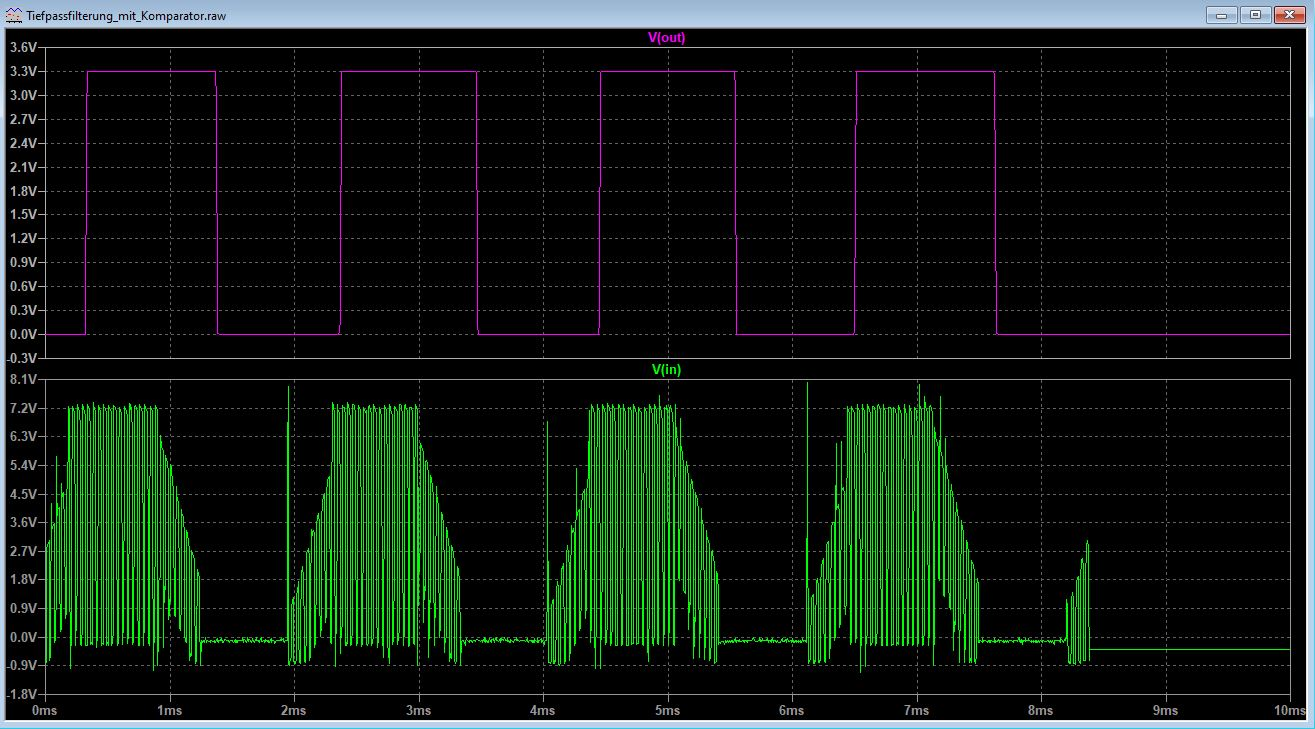
\includegraphics[width=.99\textwidth]{sec4/images/Signaldarstellung} 
\centering
\captionsetup{width=.95\textwidth}
\caption[Signaldarstellung]{Gemessenes Ausgangssignal des \ac{ESC}s Vin (grün) bei schneller Fahrt und Darstellung des gewünschten Ausgangssignals Vout (pink) mit dem Schaltungssimulationstool LTspice XVII}\centering
\label{fig:Signaldarstellung}
\end{figure}

Die Grundidee der Drehzahlregelung ist es, bei den verwendeten \acp{BLDCMot} die Drehzahl über die Variation der Frequenz einzustellen. Dabei soll, die Anzahl der steigenden oder fallenden Flanken des umgeformten PWM-Signals mit Hilfe eines Zählers in einem gewissen Zeitbereich bestimmt werden. Hierzu wird pro ESC jeweils eine Phase in die genannte Tiefpass-/Komparatorschaltung geführt. Mit Hilfe der umgeformten Signale kann anhand einer definierten softwaretechnischen Skalierung der Zählerwerte, eine dazugehörige definierte Drehzahl vorgegeben werden. In Folge der Spannungsabhängigkeit der Motoren, ist es notwendig, eine Verringerung der Drehzahl aufgrund der Entladung des Akku-Packs schnellstmöglich zu erfassen, um dadurch die Effektivität der BLDC-Motoren über einen längeren Zeitraum aufrechtzuerhalten. \vspace{11pt}

Das vorgestellte Messprinzip bietet somit den Vorteil, dass je nach Bedarf und Genauigkeit eine selbstbestimmte Signalaufbereitung möglich ist, welche zu jeder Zeit umprogrammiert werden kann.  Ebenfalls werden die Schaltungen auf einer ohnehin vorgesehenen Verteilerplatine aufgelötet, dabei kann der Platz effektiv genutzt werden und es werden weniger lange Verbindungsdrähte benötigt. Es gilt zu erwähnen, dass auch bei dieser Methode eine Erfassung der Drehrichtung möglich ist. Dazu müssten zwei Phasen pro Motor vermessen werden um eine Vorzeichenänderung der Spannung zu detektieren. Allerdings wäre es auch bei diesem Messprinzip nicht möglich den Stillstand von 0rpm zu erfassen. Aufgrund der nicht Notwendigkeit der Drehrichtungserfassung wird hierauf nicht näher eingegangen.\vspace{11pt}

Da auch bei diesem Messprinzip ein gewisser Planungs-, Konstruktions- und Montageaufwand erforderlich ist, gilt es also abzuwägen, welche dieser beiden Methoden die meisten Vorteile für das Gesamtprojekt bietet. Das Projektteam entscheidet sich nach Betrachtung der Vor- und Nachteile für die Realisierung einer Tiefpass- /Komparatorschaltung, da der Arbeits- und Zeitaufwand zunächst als geringer eingestuft wird. Zum anderen besteht im Projektteam das Interesse, eine eigene Schaltung zu planen und zu entwerfen. Die Umformung der von ESCs ohnehin bereitgestellten Signale (Vin) bietet sich für die Realisierung dieser Methode an. Als weitere Gründe werden neben des geringeren Materialaufwands, auch die komplizierte und fehlerbehaftete Montage der Magnetklötze, sowie die nicht Notwendigkeit der Drehrichtungserfassung, welche mit dem Hallsensor leichter zu erfassen wäre, genannt. Zusätzlich bietet die flexible und selbstbestimmte Signalaufbereitung mit Hilfe der umgeformten Signale durch softwaretechnische Maßnahmen Vorteile in der Flexibilität.\vspace{11pt}

\subsubsection{Hardware für die Drehzahlmessung}\label{Sec4Sub5Sub3}

In diesem Abschnitt wird die Entwicklung der Schaltung zur Drehzahlmessung beschrieben. Dabei wird sowohl auf die Probleme die während der Schaltungsentwicklung auftraten sowie auf deren Behebung eingegangen. Damit das von den ESCs gelieferte hochfrequenten Eingangssignals in ein gleichmäßig definiertes PWM-Signal umgesetzt werden kann, bedarf es der im vorherigen Abschnitt erörterten Entwicklung einer Tiefpass-/ Komparatorschaltung. Es soll deutlich gemacht werden, welche Bauteile verwendet werden und welche Aufgaben sie in der Schaltung erfüllen. Zur Entwicklung und Simulation der Drehzahlmessschaltung wird das Schaltungssimulationstool LTspice XVII verwendet. Zur Erstellung des Platinenlayouts wird die Freeware BlackBoard Circuit Designer verwendet.\vspace{11pt}

Zu Beginn wird die Schaltung für einen ESC in LTspice realisiert. Der in LTspice erstellte Schaltplan zur Drehzahlmessung ist in Abbildung 48 abgebildet und dient als Überblick der verwendeten Bauteile mit den entsprechenden Kennwerten. Es gilt zu erwähnen, dass der Spannungsteiler (R5, R6, R7, R8) zwischen Vref und dem invertierenden Operationsverstärkereingang IN- nur einmal realisiert werden muss, worauf im weiteren noch detallierter eingegangen wird.

\begin{figure}[H] %H für Positionierung hier
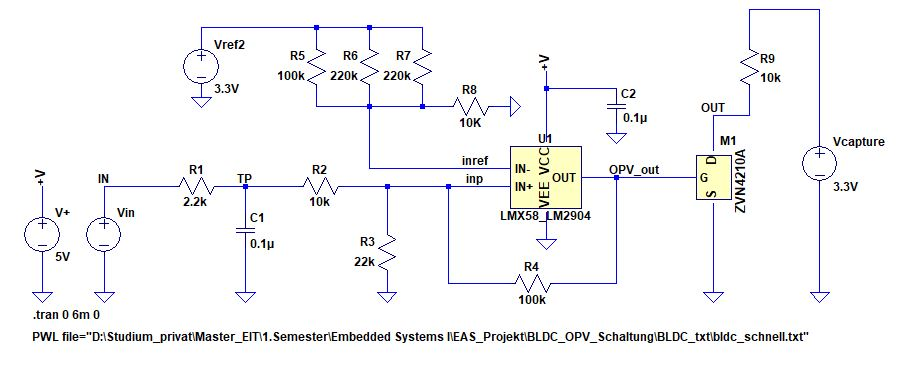
\includegraphics[width=.95\textwidth]{sec4/images/Schaltungsaufbau} 
\centering
\captionsetup{width=.95\textwidth}
\caption[Schaltungsaufbau]{Darstellung der geplanten Schaltung in LTspice XVII für einen ESC}\centering
\label{fig:Schaltungsaufbau}
\end{figure}

Zunächst simuliert die Spannungsquelle Vin einen ESC und stellt das von dort kommende hochfrequente Signal, welches bereits in Abbildung 48 (grüner Spannungsverlauf) gezeigt wurde, bereit. Die Signale werden vor Beginn der Schaltungsentwicklung an einer Phase eines ESCs mit dem Oszilloskop gemessen worden. Hierzu wird das Fahrzeug auf den entsprechenden Modell-Prüfstand gestellt und einmal mit hoher und einmal mit niedriger Drehzahl gesteuert. Es gilt zu erwähnen, dass die erfassten Signale für schnelle und langsame Fahrt nicht den maximalen und minimalen Drehzahlen, sprich \glqq{}FULLTHROTTLEg\grqq{} und \glqq{}STOPTHROTTLE \grqq{} entsprechen. Das verwendete Oszilloskop (DSO-X 3034A) bietet dabei die Möglichkeit die gemessenen Ausgangssignale als csv-Datei auf einem USB-Stick zu speichern. Das gespeicherte csv-File kann daraufhin als PWL-File in LTspice importiert und einer Spannungsquelle übergeben werden (rechter Mausklick auf die Spannungsquelle - PWL FILE - Pfad des csv-File auswählen).\vspace{11pt}

Das ungefilterte Ausgangssignal (siehe Vin Abbildung 47) besitzt sowohl bei schneller als auch bei langsamer Fahrt eine Frequenz von ca. 23 kHz. Um die hohen Frequenzanteile des Signals im ersten Schritt zu filtern, wird zunächst ein Tiefpass erster Ordnung benötigt. Die Dimensionierung des Tiefpasses erfolgt mit einem 1,1 kOhm Widerstand R1 und einem 100 nF Kondensator C1. Dabei beträgt die Grenzfrequenz des Tiefpasses ca. 1,45 kHz und kann mit der Formel(2) berechnet werden. Der aus der Simulation resultierende Spannungsverlauf (Abbildung 49) sowie der am Oszilloskop gemessene Spannungsverlauf (Abbildung 50) nach der Tiefpassfilterung sind nachfolgend dargestellt.\vspace{11pt}

\begin{equation}\label{eq1}
f_G = \frac{ 1 }{2 \cdot \pi \cdot R1\cdot C1 }
\end{equation}

\begin{figure}[H] %H für Positionierung hier
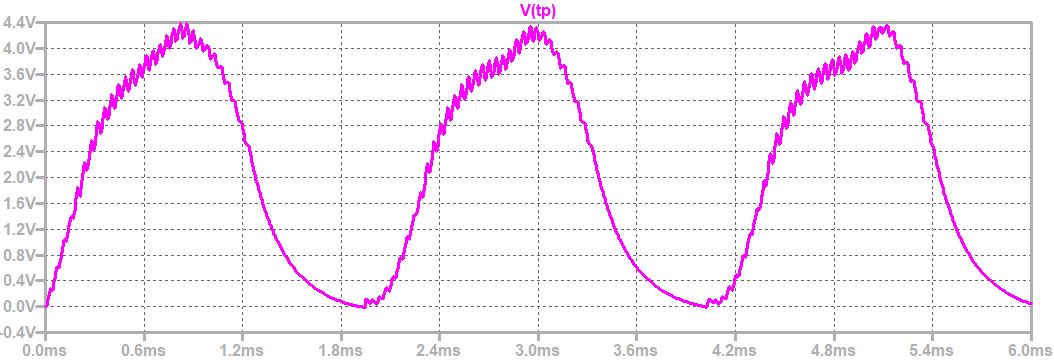
\includegraphics[width=.90\textwidth]{sec4/images/Spannungsverlauf_TP} 
\centering
\captionsetup{width=.95\textwidth}
\caption[Spannungsverlauf\_TP]{Beispielhaftes Simulationsergebnis des Ausgangssignal nach Tiefpassfilterung bei schneller Fahrt}\centering
\label{fig:SpannungsverlaufTP}
\end{figure}

\begin{figure}[H] %H für Positionierung hier
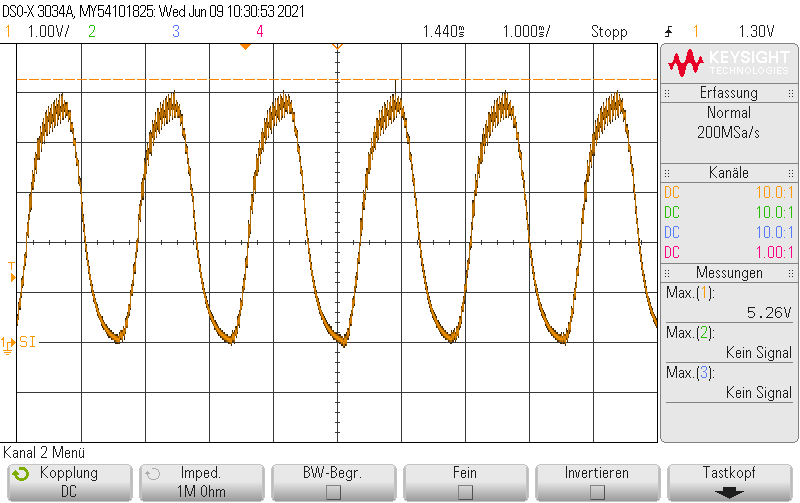
\includegraphics[width=.90\textwidth]{sec4/images/TP} 
\centering
\captionsetup{width=.95\textwidth}
\caption[TP]{Gemessenes Ausgangssignal nach Tiefpassfilterung (Messpunkt TP) bei schneller Fahrt (330.000}\centering
\label{fig:SpannungsverlaufTP}
\end{figure}

Das zentrale Bauelement der Schaltung ist ein von Texas Instruments (TI) hergestellter Operationsverstärker LM358A. Hierbei handelt sich um einen Standard Dual Operational Amplifier (op amp), welcher im Single-Supply betrieben wird. Der Operationsverstärker (OPV) wird zunächst mit einer Versorgungsspannung V+ von 3.3V, welche vom Pin X.Y geliefert wird, betrieben. Für die Drehzahlmessung wird jeweils eine Schaltung für das Signal des linken und des rechten ESCs benötigt. Der verwendete OPV ermöglicht es beide Signale (ESC links, rechts) in einem Modul zu verarbeiten. Dazu besitzt er zwei invertierende Eingänge (IN1-, IN2-) und zwei nicht-invertierende Eingänge (IN1+, IN2+) sowie zwei Ausgänge (OUT1, OUT2) (siehe Abbildung 50). Dadurch kann auf der Verteilerplatine zusätzlicher Platz eingespart werden.

\begin{figure}[H] %H für Positionierung hier
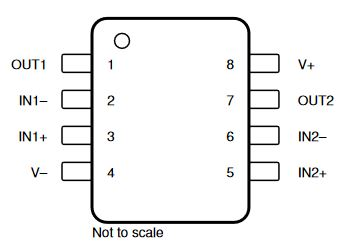
\includegraphics[width=.50\textwidth]{sec4/images/OPV_Pinbelegung} 
\centering
\captionsetup{width=.95\textwidth}
\caption[OPV\_Pinbelegung]{Darstellung der Pinbelegung des verwendeten OPV LM358A}\centering
\label{fig:Schaltungsaufbau}
\end{figure}


Da der OPV in der Schaltung als Komparator verwendet wird, müssen einige schaltungstechnische Maßnahmen, wie z.B. ein Spannungsteiler mit Rückführwiderstand hinzugefügt werden. Die Realisierung des Spannungsteilers erfolgt mit den Widerständen R2 (10 kOhm), R3 (22 kOhm) sowie einem Rückführwiderstand R4 (100 kOhm) vom Ausgang des OPV kommend. Die Kombination der Widerstände wurde durch Verwendung des Schaltungssimulationstools (LTspice XVII) und anhand der verfügbaren Widerstandsgrößen ermittelt.\vspace{11pt}

Grundsätzlich vergleicht ein Komparator ständig seine Eingangsgrößen (IN+, IN-) und zeigt digital an, welcher Eingang die größere Spannung besitzt. Da ein Operationsverstärker einen nahezu unendlichen Verstärkungsfaktor besitzt, reicht eine geringe Eingangsspannungsdifferenz, um den Ausgang in die Sättigung gehen zu lassen. Der hier verwendete OPV LM358A besitzt einen open-loop voltage gain von 100V/mV. Allerdings kann der Ausgang des OPV nur Werte im Bereich der Zustände V+ und V- annehmen. Versorgt man den Operationsverstärker mit einer Versorgungsspannung von +3,3 V und legt V- auf Masse, so erhält man im Idealfall am Ausgang ein TTL-Signal mit der maximalien Höhe der Versorgungsspannung zur digitalen Weiterverarbeitung. Sind beide Eingangsspannungen annähernd gleich, so kippt der Ausgang bei der kleinsten Störung oder Veränderung hin und her. Um dieses Problem zu vermeiden, wird eine Hysterese eingebaut. Das bedeutet, dass bei erreichen einer bestimmten Referenzspannung oder einem bestimmten Pegel am invertierenden Eingang eingeschaltet, und bei einem wiederholten erreichen der Referenzspannung wieder ausgeschaltet wird (siehe Abbildung 52 Schnittpunkte IN+ (grün) und IN- (blau)).\vspace{11pt}

Wie bereits erwähnt kann der Ausgang des OPV im Idealfall seine Versorgungsspannung V+ und V- annehmen, da aber das verwendete OPV-Modell lediglich über eine Single Supply Funktion und nicht über eine Rail-to-Rail Funktion verfügt, bleibt die max. Ausgangsspannung stets unter der angeschlossenen Versorgungsspannung. Hierzu ist in Abbildung 52 der nach unten abweichende Spannungsverlauf OPV out (gelb) dargestellt, die Versorgungsspannung bei dieser Aufnahme beträgt V+ 5V.\vspace{11pt}

Da zu Beginn der Schaltungsentwicklung in der Simulation jedoch keine signifikanten Abweichungen festgestellt werden, wird der OPV zunächst mit einer Spannung V+ von 3,3V versorgt. Erst eine Messung mit dem Ozilloskop macht ein deutlich abweichendes Verhalten im Vergleich zur Simulation deutlich. Es werden am Ausgang des OPV bei FULLTHROTTLE lediglich 2,08V und bei \glqq{}STOPTHROTTLE \grqq{} nur ca. 0,1V gemessen. Dies führt dazu, dass insbesondere im niedrigen Drehzahlbereich, sprich ab einer Unterschreitung der Referenzspannung Vref von 540 mV kein PWM-Signal mehr erzeugt wird. Darüber hinaus ist im zugehörige Datenblatt des verwendeten Mikrocontrollers ersichtlich, dass die Timer2 Capture Input Pins(P0.24 Antrieb rechts, P0.25 Antrieb links) eine Mindestspannung von 2,0V benötigten um zuverlässig Signale verarbeiten zu können. Da dieser Spannungswert insbesondere im niedrigen Drehzahlbereichs nicht erreicht wird, ist die Schaltung in dieser Form für den Anwendungszweck nicht ausreichend.\vspace{11pt}

\begin{figure}[H] %H für Positionierung hier
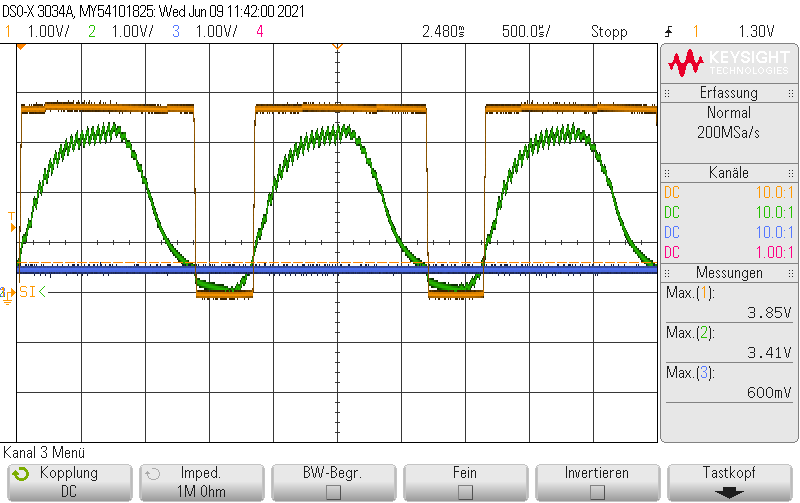
\includegraphics[width=.95\textwidth]{sec4/images/inp_inref_opv_out} 
\centering
\captionsetup{width=.95\textwidth}
\caption[inp\_inref\_opv\_out]{Beispielhafte Messung des OPV Ausgangssignals OPV out (gelb) bei einer Versorgungsspannung von V+ 5,0V Single Supply,  IN+ (grün), Vref am IN- (blau)}\centering
\label{inpInrefOpvOut}
\end{figure}

Als erste Lösung der Problematik wird versucht die Spannungsversorgung des OPV auf V+ 5V zu erhöhen. Durch die Erhöhung der Versorgungsspannung kann grundsätzlich eine höhere Ausgangsspannung erzielt werden, dennoch gilt dies weiterhin nur für größere Drehzahlbereiche. Eine Spannung größer 2,0 V, wird vor allem im Bereich der niedrigeren Drehzahlen nach wie vor nicht zuverlässig erreicht.\vspace{11pt}


Damit eine zuverlässige Bereitstellung einer konstanten Signalspannung für die Timer2 Capture Input Pins am Mikrocontroller größer als 2,0 V erreicht werden kann, wird ein zusätzlicher n-Kanal Mosfet ZVN4210A am Ausgang des OPV implementiert. Der in Abbildung 49 dargestellte Widerstand R9 (10 kOhm) vor dem Drain-Anschluss des Mosfets, stellt den intern einstellbaren Pull-up Widerstand der Timer2 Capture Input Pins des Mikrocontrollers dar. Je nach Konfiguration können diese zu- abgeschalten werden. Im Zuge der Entwicklung wird der Pull-up Widerstand R9 auf einem Whiteboard angebracht und entsprechend verdrahtet.\vspace{11pt}

Zur Bereitstellung der am invertierenden OPV-Eingang (IN-) benötigten Referenzspannung, auch Schwellspannung genannt, wird ein zusätzlicher Spannungsteiler mit einer vom PIN X.Y. kommenden +3,3V Spannungsversorgung vorgeschalten. Der Spannungsteiler besteht aus drei parallel geschaltenen Widerständen R5 (100 kOhm), R6 und R7 (220 kOhm) in Reihe zum Widerstand R8 (10 kOhm). Die dadurch bereitgestellte Spannung beträgt in etwa 540mV.  Wie bereits erwähnt, ermöglicht die Referenzspannung (Vinref) zusammen mit dem Eingangssignals am nicht-invertierenden Eingang (Vinp), dass durchschalten von V+ am OPV Ausgang. Die bereitgestellte Referenzspannung von 540mV ist in der Theorie ausreichend um für alle Drehzahlen ein zuverlässiges PWM-Signal zu erzeugen. In der Praxis treten dennoch wiederholt Probleme auf. Die Problematik sowie deren Lösung werden im nachfolgenden Abschnitt 4.5.4 \glqq{}Ausblick Schaltungserweiterung\grqq{} beschrieben. \vspace{11pt}

In Abbildung 53 links, ist die auf der Verteilerplatine befindliche Drehzahlmessschaltung im Original zu sehen. Auf der rechten Seite von Abbildung 53 befindet sich der mit dem Programm BlackBoard Circuit Designer erstellte zugehörige Stromverlaufsplan, welcher eine schnelle Übersicht ermöglicht. Die grünen Verbindungen stellen die Pfade zwischen Vin (Eingangssignal von den ESCs) bis zum OPV Eingang IN+ dar, Vref (gelb) Pfad der Referenzspannung zu den invertierenden Eingängen IN1-, IN2- des OPV. Der Pfad zur Spannungsversorgung des OPV (V+) ist mit violett dargestellt und alle schwarzen Verbindungen stellen GND-Verbindungen dar. Zuletzt kann der Verlauf der Ausgangsspannung des OPV out anhand der roten Verbindungen nachvollzogen werden. 

\begin{figure}[H] %H für Positionierung hier
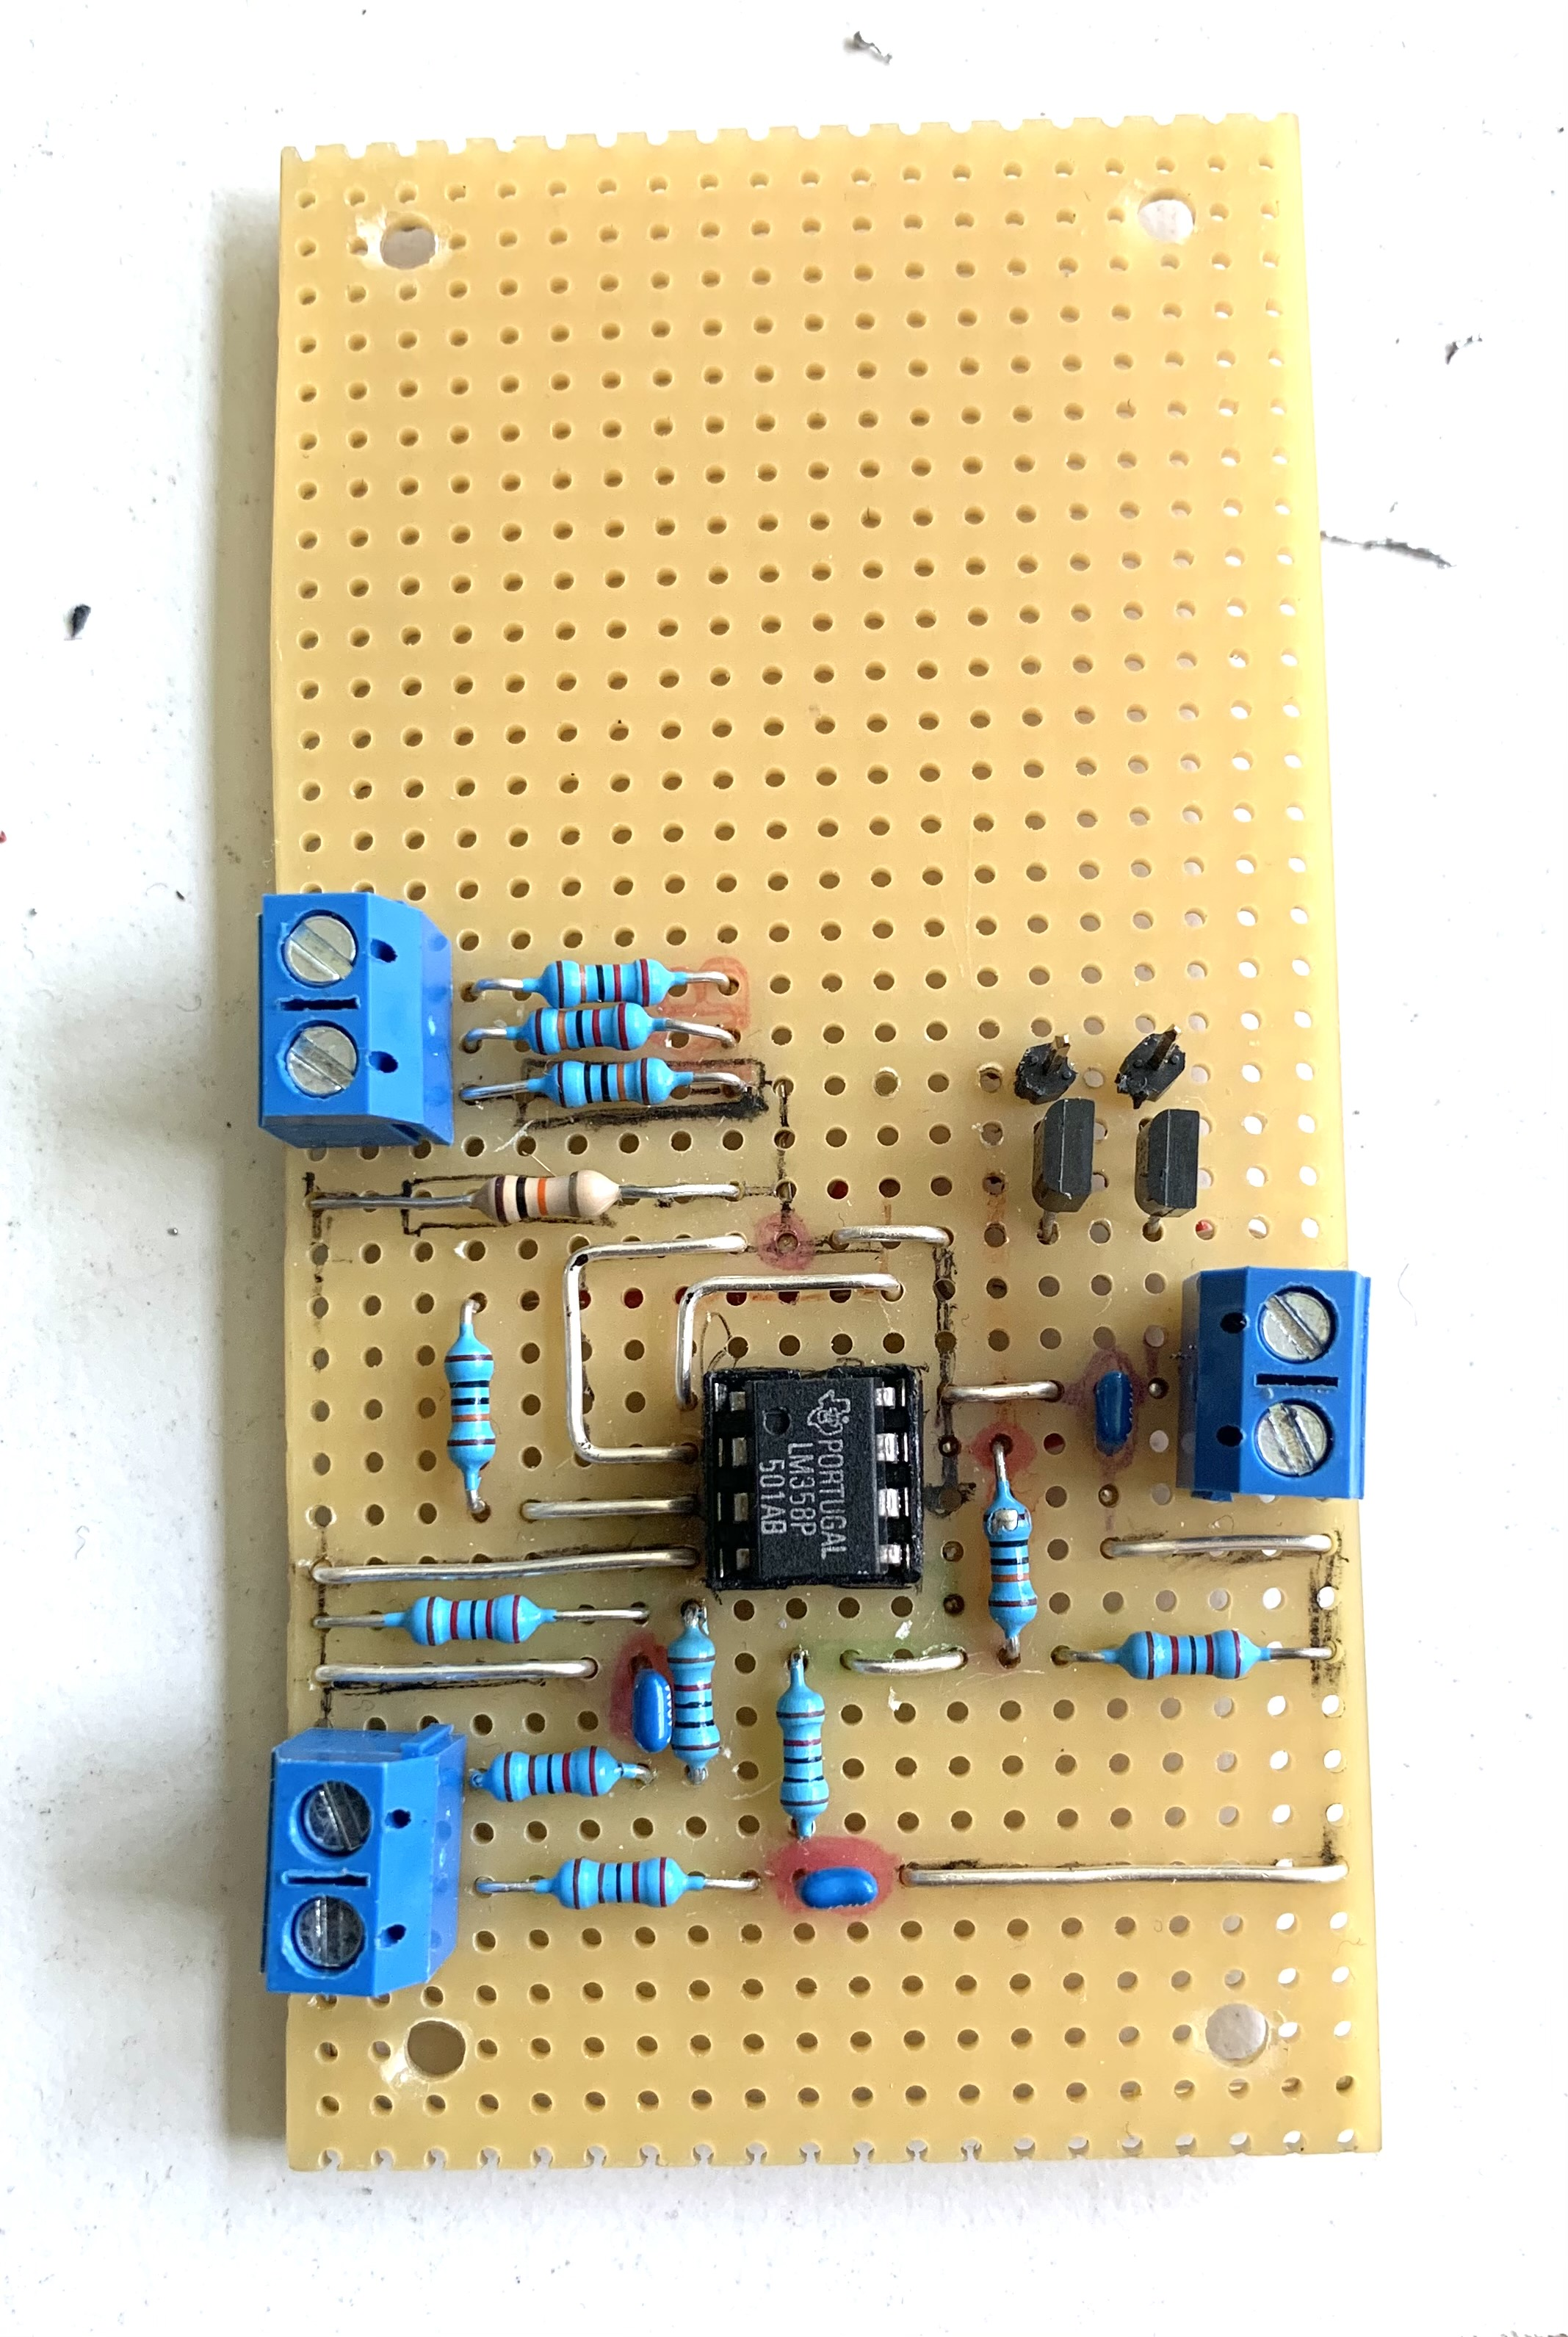
\includegraphics[width=.45\textwidth]{sec4/images/Platine} 
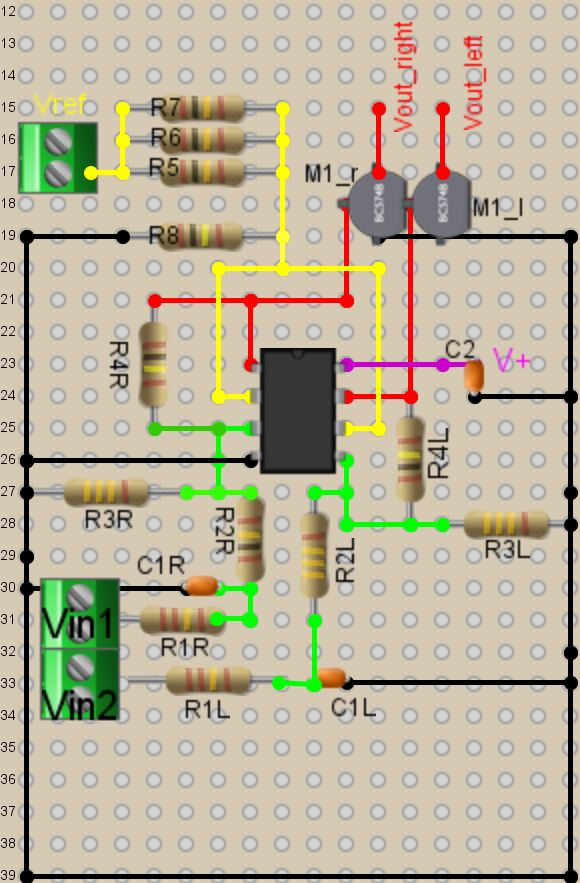
\includegraphics[width=.40\textwidth]{sec4/images/Platinendesign}
\captionsetup{width=.95\textwidth}
\centering
\caption[Schaltungsaufbau\_mit\_Mosfet]{Schaltung Drehzahlmessung auf Verteilerplatine (links), Übersicht Platinenaufbau mit markierten Stromverlaufspfaden}\centering
\label{fig:Schaltungsaufbau}
\end{figure}


\subsubsection{Ausblick Schaltungserweiterung}\label{Sec4Sub5Sub4}
 
Nachdem die Referenzspannung Vref in der Schaltung so dimensioniert ist, sodass in der Theorie alle Drehzahlen zuverlässig als eindeutiges PWM-Signal dargestellt werden können, treten in Praxis noch Probleme auf. Denn nach Messung der Spannung mit dem Oszilloskop am PIN X.Y, wurden anstelle der exakten +3,3V, Spannungen bis zu 3,65V gemessen. Dies führt zu einer schwankenden Referenzspannung von etwa 540mV bis 600mV. Das Problem, Drehzahlen im sehr niedrigen Drehzahlbereich insbesondere im \glqq{}STOPTHROTTLE \grqq{}, 1,09 ms bis 1,10ms ton-Zeit, werden nicht immer zuverlässig als eindeutiges PWM-Signal dargestellt, da die Referenzspannung keine eindeutigen Schnittpunkte mit dem Eingangssignal besitzt (siehe Abbildung 54).\vspace{11pt}
 
\begin{figure}[H] %H für Positionierung hier
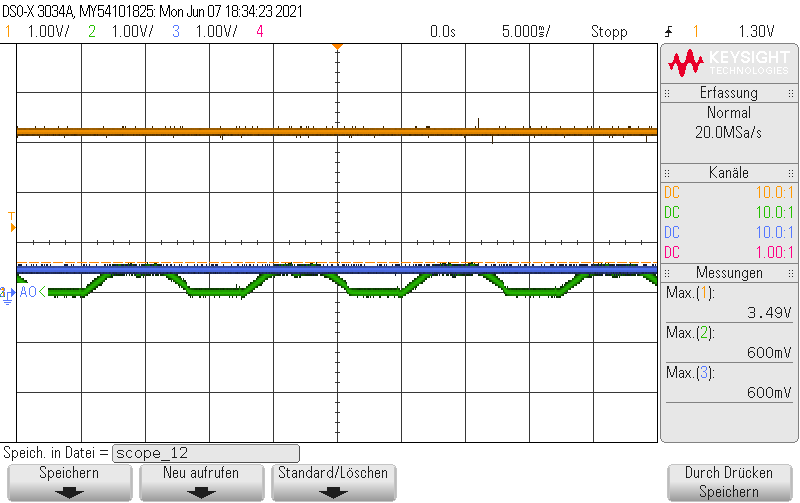
\includegraphics[width=.95\textwidth]{sec4/images/Problematik_stop_throttle} 
\centering
\captionsetup{width=.95\textwidth}
\caption[Problematik\_stop\_throttle]{Beispielhafte Messung bei nicht übereinstimmenden Schaltschwellen für das Eingangssignal - Folge: kein Schalten des OPV möglich }\centering
\label{fig:ProblematikStopThrottle}
\end{figure}

Eine mögliche Lösung der Problematik, ist die Erweiterung des Spannungsteiler zur Einstellung der Referenzspannung vor dem invertierenden Eingang des OPV um einen n-Kanal Mosfet gegen Masse (siehe Abbildung 55). Diese Maßnahme ermöglicht es, die Referenzspannung, für hohe und niedrige Drehzahlen flexibel anzupassen um ein zuverlässiges Ausgangssignal zu erhalten.\vspace{11pt}

Durch die Vorgabe eines bestimmten Modus, in der Schaltung als MCU-Mode bezeichnet, kann durch die Definierung von zwei Drehzahlbereichen, beispielsweise ton-Zeit 1,09ms bis 1,43ms für langsame Drehzahlen eine Referenzspannung zwischen 400mV-500mV eingestellt werden. Der Vorteil ist, dass man dadurch einen bestimmten Tolerenzbereich für Schwankungen der Versorgungspannung vom Pin erzeugt und die Schaltung dadurch weniger anfällig für Abweichungen ist.\vspace{11pt}

Softwareseitig kann hierzu eine Interrupt Service Routine programmiert werden, welche bei erkennen des niedrigen Drehzahlbereichs einen weiteren Pin des Mikrocontrollers so schaltet, sodass dieser die Gate Spannung des Mosfets liefert und den Widerstand R7 folglich gegen Masse schaltet. Durch den zusätzlichen parallelen Widerstand kann die Referenzspannung verringert werden. Zur Bestimmung der Widerstandswerte für R5, R6 und R7 können folgende Formeln (3), (4) verwendet werden.\vspace{11pt}

\begin{equation}\label{eq1}
V_{ModeLow} = \frac{ R6 }{R6 + R5 }\cdot 3,3V
\end{equation}

\begin{equation}\label{eq1}
V_{ModeHigh} = \frac{ R2 || R3 + R_{DSON} }{R2 || R1 + R_{DSON} + R5 }\cdot 3,3V
\end{equation}

\begin{figure}[H] %H für Positionierung hier
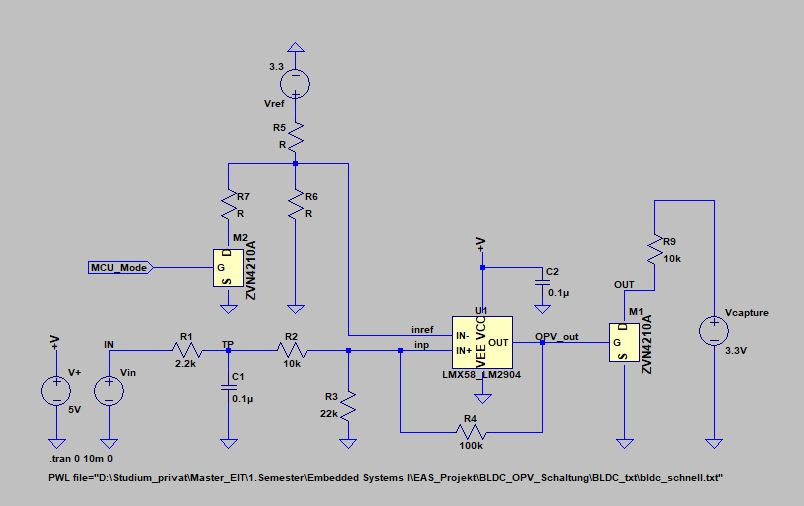
\includegraphics[width=.99\textwidth]{sec4/images/Schaltungserweiterung} 
\centering
\captionsetup{width=.95\textwidth}
\caption[Schaltungserweiterung]{Schaltungsaufbau mit einstellbarer Referenzspannung für die invertierenden Eingänge IN1-, IN2-}\centering
\label{fig:Schaltungserweiterung}
\end{figure}

\subsubsection{Programmierung des Drehzahlmessungsbausteins}\label{Sec4Sub5Sub4}

Damit das durch die Schaltung bereitgestellte PWM-Signal vom Mikrocontroller softwareseitig erfasst werden kann, wird grundsätzlich ein Timer Capture Register benötigt. Dieses Register speichert bei einem Ereignis, bspw. das Auftreten einer steigenden Flanke, am angeschlossenen Input Pin den aktuellen Timerwert und kann daraufhin einen Interrupt auslösen.\vspace{11pt}

Der Softwarebaustein zur Drehzahlerfassung ist in zwei Dateien unterteilt, die Dateien \glqq{}rpmMeas.c\grqq{} und \glqq{}rpmMeas.h\grqq{}. Die Datei \glqq{}rpmMeas.h\grqq{} enthält alle relevanten Bibliotheken und Prototypen für die Datei \glqq{}rpmMeas.c\grqq{}. Hier werden die beiden Channel zur Erfassung der Daten auf das Timer Caputure Register 0 (rechter Antrieb, \glqq{}kCTIMER\_Caputre\_0\grqq{}) und auf das Timer Capture Register 1 (linker Antrieb, \glqq{}kCTIMER\_Capture\_1\grqq{}) festgelegt. Bei dem verwendeten Mikrocontroller entspricht dies den Pins P0.25 (rechts) und P0.24 (links). Der Pin P0.25 wird auf der Controllerplatine über den Pin 4 und der Pin P0.24 über den Pin 6 der Buchsenleiste J13 nach außen geführt.\vspace{11pt}

\begin{figure}[H] %H für Positionierung hier
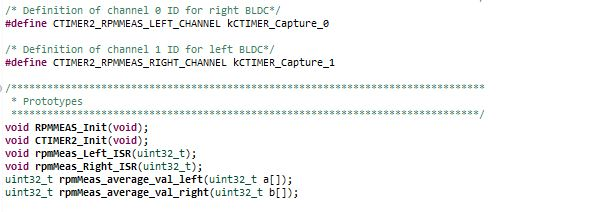
\includegraphics[width=.80\textwidth]{sec4/images/rpm_defines} 
\centering
\captionsetup{width=.95\textwidth}
\caption[rpm\_defines]{Relevante Zeilen der Datei \glqq{}rpmMeas.h\grqq{} zur Initialsierung des Timers 2 für das PWM Signal sowie Prototypen }\centering
\label{fig:Schaltungsaufbau}
\end{figure}

Die Datei \glqq{}rpmMeas.c\grqq{} enthält die Funktionen zur Initialisierung der für die Verwendung der Drehzahlerfassung notwendigen Controller-Peripherie als auch die Definition und Initialisierungen der notwendigen Parameter zur Erfassung und Berechnung der benötigten Drehzahlwerte (siehe Abbildung 57).  \vspace{11pt}


In der Funktion RPMMEAS\_Init wird zuerst die Funktion CTIMER2\_Init aufgerufen, welche unter anderem die beiden vorher festgelegten Kanäle des Timers C2 (\glqq{}kCTIMER\_Caputre\_0\grqq{} und \glqq{}kCTIMER\_Capture\_1\grqq{}) initialisiert. Bei der Initialisierung der Capture Channel (CTIMER\_SetupCapture) wird das entsprechende Ereignis, bei dem ein Capture stattfinden soll, festgelegt. In diesem Fall wird der Trigger der beiden Kanäle auf die steigende Flanke gesetzt (\glqq{}kCTIMER\_Capture\_RiseEdge\grqq{}) und im Anschluss der Enable für die Capture Interrupts auf 1 gesetzt. \vspace{11pt}

Damit beim Auftreten einer steigenden Flanke des PWM-Signals, ein Interrupt Flag ausgelöst werden kann, benötigt man bei MCUxpresso zunächst einen cTimer\_callback\_table. Der Callback-Table wird als Parameter initialisiert und muss mit den verwendeten Interrupt Service Routinen rpmMeas\_Left\_ISR und rpmMeas\_Right\_ISR verknüpft werden. Der Callback-Table wird als Pointer-Array in der CTIMER2\_Init der Funktion CTIMER\_RegisterCallBack übergeben. Bei einer Callback-Funktion auch Rückruffunktion genannt, wird einer Funktion als Parameter eine andere Funktion übergeben. Des weiteren muss in der RegisterCallBack-Funktion der Typ des Callbacks festgelegt werden. In diesem Fall wird der Callback als \glqq{}kCTIMER\_MultipleCallback\grqq{} festgelegt, was bedeutet, dass pro Channel ein Callback durchgeführt werden kann. Zuletzt wird in der CTIMER2\_Init der Timer C2 gestartet.\vspace{11pt}

Nach Vollendung der Initialisierungsfunktionen des CTIMER2\_Init werden in der Funktion RPMMEAS\_Init zusätzlich die Pins P0.24 (Antrieb links) und P0.25 (Antrieb rechts) für die Verwendung als PWM-Input Capture Pin des Timercs C2 konfiguriert.

\begin{figure}[H] %H für Positionierung hier
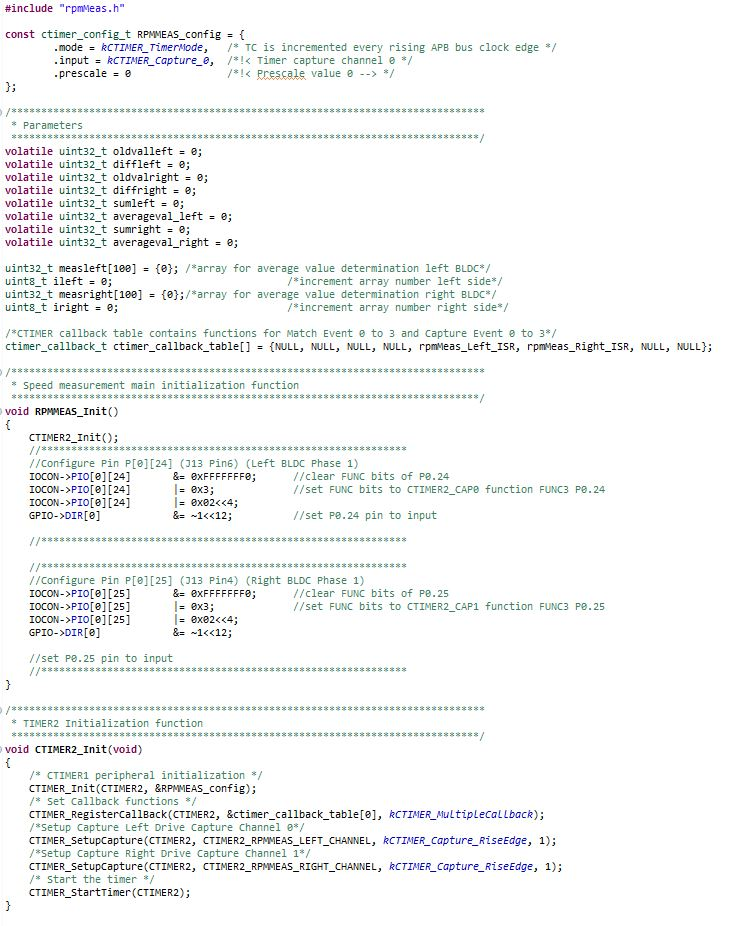
\includegraphics[width=.90\textwidth]{sec4/images/rpmmeas_init_ctimer2_init} 
\centering
\captionsetup{width=.95\textwidth}
\caption[rpmmeas\_init\_ctimer2\_init]{Funktionen RPMMEAS\_Init und CTIMER2\_Init in der Datei Relevante Zeilen der Datei \glqq{}rpmMeas.c\grqq{}}\centering
\label{fig:rpmmeasInitCtimer2Init}
\end{figure}


Zur Erfassung der Drehzahl wird im Programm jeweils eine Interrupt Service Routine rpmMeas\_Left\_ISR und rpmMeas\_Right\_ISR für die jeweilige Antriebsseite benötigt. Sobald eine steigende Flanke getriggert wird, wird durch das setzen eines Interrupt Flags die ISR ausgelöst und die vom Timer C2 erfasste Zeit zwischen zwei steigenden Flanken mit dem Befehl CTIMER\_GetTimerCountValue an die ISR übergeben. Die aktuell gemessene Zeit wird mit der vorherig gemessenen Zeit (oldvalright, oldvalleft) subtrahiert und die resultierende Differenz (diffright oder diffleft) den Arrays zur Mittelwertberechnung (measright[], measleft[]) übergeben.\vspace{11pt}  


\begin{figure}[H] %H für Positionierung hier
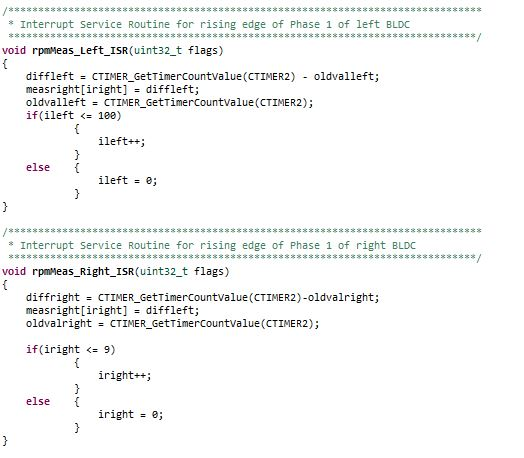
\includegraphics[width=.62\textwidth]{sec4/images/isr} 
\centering
\captionsetup{width=.95\textwidth}
\caption[isr]{Interrupt Service Routinen zur Erfassung der Capture Daten }\centering
\label{fig:isr}
\end{figure}

Die Werte des in den Arrays (\glqq{}measright[]\grqq{} und \glqq{}measleft[]\grqq{}) abgelegten Werte, werden daraufhin der Funktion \glqq{}rpmMeas\_average\_val\_right()\grqq{}, \glqq{}rpmMeas\_average\_val\_right()\grqq{} übergeben. Dabei wird aus zehn erfassten Werten der Mittelwert gebildet. Der berechnete Mittelwert \glqq{}averageval\_right\grqq{}, \glqq{}averageval\_left\grqq{} wird in den weiteren Schritten zur Bestimmung der Drehzahlregelung benötigt. 


\begin{figure}[H] %H für Positionierung hier
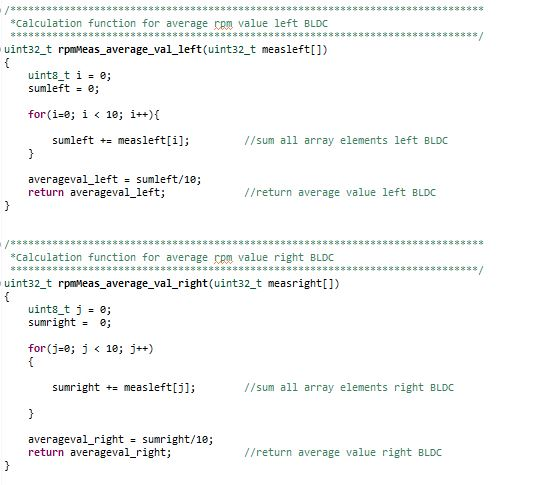
\includegraphics[width=.62\textwidth]{sec4/images/calculation} 
\centering
\captionsetup{width=.95\textwidth}
\caption[calculation]{Funktionen zur Berechnung des Mittelwerts aus den erfassten Capture Daten }\centering
\label{fig:calculation}
\end{figure}

Im letzten Abschnitt der RPMMEAS\_Init werden an die zwei Funktionen \glqq{}rpmMeas\_average\_val\_left\grqq{} und \glqq{}rpmMeas\_average\_val\_right\grqq{} die Arrays mit den erfassten Drehzahldaten übergeben. Aus den erfassten Daten kann daraus der Mittelwert \glqq{}averageval\_left\grqq{} bzw. \glqq{}averageval\_right\grqq{} gebildet werden und im weiteren einer entsprechenden Funktion zur Drehzahlregelung weitergegeben werden.


\newpage